\documentclass[journal]{IEEEtran}

% ============== Packages ==============
\usepackage{amsmath,amsfonts,amssymb}
\usepackage{algorithmic}
\usepackage{algorithm}
\usepackage{array}
\usepackage[caption=false,font=normalsize,labelfont=sf,textfont=sf]{subfig}
\usepackage{textcomp}
\usepackage{stfloats}
\usepackage{url}
\usepackage{verbatim}
\usepackage{graphicx}
\usepackage{cite}
\usepackage{booktabs}
\usepackage{multirow}
\usepackage{color}
\usepackage{xcolor}

% Graphics path
\graphicspath{{figs/}}

% Hyphenation
\hyphenation{op-tical net-works semi-conduc-tor IEEE-Xplore}

% ============== Document ==============
\begin{document}

% ============== Title ==============
\title{SA-FLQ: System-Aware Federated Learning with Adaptive Low-Bitwidth Quantization for Maritime Edge Computing}

% ============== Authors ==============
\author{
    \IEEEauthorblockN{Jiahong Ning\IEEEauthorrefmark{1}, 
    Tingting Yang\IEEEauthorrefmark{1}, 
    Ping Feng\IEEEauthorrefmark{1}, and 
    Xiufeng Zhang\IEEEauthorrefmark{1}}
    \IEEEauthorblockA{\IEEEauthorrefmark{1}Dalian Maritime University, Dalian, China}
    \thanks{J. Ning is a Student Member, IEEE. T. Yang is a Member, IEEE.}
    \thanks{Corresponding author: Tingting Yang (yangtt@dlmu.edu.cn)}
}

% ============== Headers ==============
\markboth{IEEE Transactions on Mobile Computing}%
{Ning \MakeLowercase{\textit{et al.}}: SA-FLQ for Maritime Edge Computing}

\maketitle

% ============== Abstract ==============
\begin{abstract}
Maritime edge computing operates under severely constrained, intermittent, and low-bandwidth communication conditions, commonly referred to as DIL environments, posing fundamental challenges for distributed machine learning. Existing federated learning approaches lack awareness of the underlying system state, resulting in inefficient resource utilization and degraded convergence. We propose SA-FLQ, a System-Aware Federated Low-bitwidth Quantization framework that integrates system-state sensing with adaptive quantization control for maritime edge scenarios.

SA-FLQ is built upon our proposed KubeEdge Wireless architecture, or KEW. This three-layer platform integrates network sensing, task orchestration, and computation. It establishes a unified system interface by defining standardized observable variables such as link bandwidth and latency, alongside controllable variables like participation sets and quantization bitwidths. Based on real-time system state feedback, SA-FLQ dynamically adjusts uplink and downlink quantization strategies through a sense-decide-execute-writeback closed-loop mechanism, achieving Pareto-optimal tradeoffs among communication overhead, computation latency, and convergence accuracy.

We validated SA-FLQ using both simulation benchmarks and a real-world oil spill detection task on a Kubernetes-based Jetson edge cluster. The results show that our method achieves up to $7.3\times$ communication compression with less than $1\%$ accuracy loss. Furthermore, it reduces per-round latency by $86\%$ compared to full-precision federated averaging.
\end{abstract}

% ============== Keywords ==============
\begin{IEEEkeywords}
System-aware federated learning, adaptive gradient quantization, maritime edge computing, KubeEdge, DIL networks, oil spill detection
\end{IEEEkeywords}

% ============================================================
%                    I. INTRODUCTION
% ============================================================
\section{Introduction}
\IEEEPARstart{T}{he} maritime industry is undergoing a significant digital transformation with an increasing number of intelligent applications being deployed at the network edge~\cite{Marine_communication_survey}. From autonomous vessel navigation and environmental monitoring to search and rescue operations, maritime services are generating vast amounts of data that require real-time processing~\cite{tInternetUnderwaterThings2021}. Traditional cloud-centric architectures face inherent limitations in maritime scenarios due to the high latency, limited bandwidth, and intermittent connectivity of maritime communication links~\cite{wei2021hybridMaritimeIoT}.

Edge computing has emerged as a promising paradigm to address these challenges by pushing computation closer to data sources~\cite{MEC_Suervey_1}. By deploying computing resources on vessels, offshore platforms, and coastal base stations, edge computing enables low-latency data processing and reduces dependency on satellite backhaul links~\cite{yang2022kubeedge}. However, edge computing in maritime environments also introduces new challenges, including resource constraints on edge devices and data isolation across distributed nodes~\cite{yangTwoStageOffloadingOptimization2020}.

The deployment of machine learning models for maritime applications such as oil spill detection and vessel classification requires collaborative training across multiple edge nodes~\cite{Edge_inttelligence}. Federated learning (FL) provides an elegant solution by enabling distributed training without centralizing raw data~\cite{mcmahan2017fedavg}. This approach not only preserves data privacy but also reduces the need for large-scale data transmission~\cite{kairouz2021fl}. However, the standard federated averaging algorithm still requires substantial communication bandwidth for model parameter synchronization, which becomes a critical bottleneck in bandwidth-constrained maritime environments~\cite{chen2020flsurvey}.

Maritime federated learning faces unique challenges that distinguish it from terrestrial scenarios~\cite{Suervey_UAV_aid_communication}. First, maritime communication relies on satellite links with high costs and limited throughput, making frequent model synchronization prohibitively expensive. Second, edge devices in maritime environments range from resource-constrained IoT sensors to powerful shipboard computing systems, leading to significant variations in processing capabilities. Third, different vessels and platforms observe different maritime conditions, resulting in highly heterogeneous local datasets with non-IID data distribution.

Existing communication-efficient FL methods such as gradient sparsification~\cite{5} and standard quantization approaches like QSGD~\cite{QSGD} have been proposed to reduce communication overhead. These methods, however, often suffer from severe accuracy degradation when applied to extreme low-bitwidth scenarios and lack optimization for the specific characteristics of maritime edge computing~\cite{lazy_aggragation}.

We propose SA-FLQ, a System-Aware Federated Low-bitwidth Quantization framework that integrates system-state sensing with adaptive quantization control for maritime edge computing. Our main contributions are as follows:

\begin{enumerate}
    \item We design the KEW platform architecture, short for KubeEdge Wireless. This three-layer edge system consists of network sensing, task orchestration, and computation layers. It establishes standardized observable and controllable variables as a unified system interface for federated learning.
    
    \item We propose SA-FLQ, a system-aware federated learning algorithm that dynamically adjusts quantization bitwidths through a sense-decide-execute-writeback closed-loop mechanism based on real-time link and node state feedback.
    
    \item We provide theoretical analysis on the convergence properties of SA-FLQ under quantization noise, establishing bounds on the communication-accuracy tradeoff.
    
    \item We validate SA-FLQ through extensive experiments on simulation benchmarks and a real-world oil spill detection task deployed on a Kubernetes-based Jetson edge cluster, demonstrating up to $7.3\times$ communication compression with less than $1\%$ accuracy degradation and $86\%$ latency reduction.
\end{enumerate}

The remainder of this paper is organized as follows. Section~\ref{sec:related} reviews related work on maritime edge computing and communication-efficient federated learning. Section~\ref{sec:system} presents the KEW platform architecture and constrained optimization formulation. Section~\ref{sec:method} describes the SA-FLQ algorithm in detail. Section~\ref{sec:experiments} presents experimental results. Finally, Section~\ref{sec:conclusion} concludes the paper.

% ============================================================
%                    II. RELATED WORK
% ============================================================
\section{Related Work}
\label{sec:related}

\subsection{Maritime Edge Computing}
The integration of edge computing with maritime networks has attracted increasing attention in recent years, driven by the growing demand for intelligent maritime services~\cite{Marine_communication_survey}. Maritime edge computing differs from terrestrial edge computing in several key aspects. First, the communication infrastructure is highly heterogeneous, consisting of satellite, shore-based, and ship-to-ship links. Second, the network topology changes dynamically due to vessel mobility. Finally, the operational environment poses unique challenges such as signal attenuation over water and limited power supply on offshore platforms~\cite{tInternetUnderwaterThings2021}.

Yang et al.~\cite{yangTwoStageOffloadingOptimization2020} proposed a two-stage offloading optimization scheme that addresses the energy-latency tradeoff in maritime IoT environments, considering the unique characteristics of maritime communication channels. Wang et al.~\cite{wangJointComputationOffloading2024} investigated joint computation offloading and resource allocation for maritime MEC with energy harvesting, demonstrating the importance of energy-aware optimization in resource-constrained maritime settings. Liu et al.~\cite{liu2022drlMaritimeUAVMEC} developed a deep reinforcement learning based approach for latency minimization in maritime UAV-assisted MEC networks, leveraging unmanned aerial vehicles as relay nodes to extend coverage.

Our previous work on KubeEdge Wireless~\cite{kubeedge_anywhere} demonstrated the feasibility of integrated communication and computing services in maritime scenarios through edge-cloud collaboration. Building upon these foundations, the current work focuses on enabling communication-efficient distributed machine learning in such bandwidth-constrained environments.

\subsection{Communication-Efficient Federated Learning}
Federated learning was first introduced by McMahan et al.~\cite{mcmahan2017fedavg} as a distributed learning paradigm that enables training on decentralized data without requiring raw data transmission. The FedAvg algorithm has since become the de facto standard for federated optimization, but its communication overhead remains a critical bottleneck, especially in bandwidth-limited scenarios~\cite{kairouz2021fl}.

To address the communication challenge, researchers have proposed various gradient compression techniques. Gradient sparsification methods such as Top-K~\cite{5} transmit only a subset of gradient elements to reduce communication volume. Quantization methods reduce the bit representation of each gradient element. QSGD~\cite{QSGD} proposed stochastic gradient quantization with provable convergence guarantees, demonstrating that 2-8 bit quantization can achieve near full-precision performance with $4{-}16\times$ compression. The Lazily Aggregated Quantized Gradient Innovation (LAQ)~\cite{lazy_aggragation} combines delayed communication with quantization, achieving multiplicative communication reduction.

FedProx~\cite{li2020fedprox} addresses the heterogeneity challenge in federated optimization by adding a proximal term to handle non-IID data and systems heterogeneity. A comprehensive survey by Chen et al.~\cite{chen2020flsurvey} provides an overview of federated learning challenges and solutions in mobile edge networks.

\subsection{Gradient Quantization Techniques}
Low-bitwidth quantization has been explored extensively for both neural network compression and communication-efficient distributed training. QSGD applies uniform stochastic quantization to gradients while providing theoretical convergence guarantees. SignSGD reduces gradients to binary representations using only the sign information, achieving maximum compression at the cost of potential accuracy loss. Our previous work FLQ~\cite{FLQ} demonstrated the effectiveness of low-bitwidth quantization in federated learning for distributed IoT systems. However, existing methods often apply uniform quantization across all layers and overlook layer-wise variation in gradient distributions.

% ============================================================
%                    III. SYSTEM MODEL
% ============================================================
\section{System Model and Problem Formulation}
\label{sec:system}

This section presents the system-aware edge architecture and mathematical formulation for maritime federated learning. We first introduce the KEW (KubeEdge Wireless) platform architecture, then define the system sensing interface through observable and controllable variables, and finally formulate the constrained optimization problem.

\subsection{KEW Platform Architecture}
We consider a maritime edge computing network consisting of a central server and $M$ edge clients distributed across vessels and offshore platforms. Each client $m \in \{1, 2, \ldots, M\}$ has a local dataset $\mathcal{D}_m$ with $|\mathcal{D}_m| = n_m$ samples. The total number of samples is $n = \sum_{m=1}^{M} n_m$.

To enable system-aware federated learning in DIL (Disconnected, Intermittent, Low-bandwidth) maritime environments, we design the \textbf{KubeEdge Wireless (KEW)} platform as a three-layer edge architecture built upon the KubeEdge framework. As illustrated in Fig.~\ref{fig:kew_layer_flow}, KEW comprises:

\begin{itemize}
    \item \textbf{Network Layer (Wireless Link):} Located at the bottom, this layer aggregates heterogeneous access technologies including satellite, microwave, and VHF links. Its core function is \textit{northbound sensing}---continuously collecting physical channel states such as effective bandwidth, round-trip time, packet loss rate, and node energy status, which are encapsulated as standardized observable variables $\boldsymbol{\omega}$.
    
    \item \textbf{Orchestration Layer (EdgeCore):} Serving as the decision hub, this layer receives control intents from the cloud or upper-layer algorithms and maps them to concrete container placement, resource quotas, and bandwidth management policies. Through metadata persistence mechanisms, it provides \textit{disconnection autonomy}---maintaining cached policies and service continuity during link outages.
    
    \item \textbf{Compute Layer (Edge Service):} Located at the top, this layer hosts training and inference workloads. It reads control parameters from the orchestration layer per training round, executes low-bitwidth computation tasks, and writes back runtime metrics (loss, latency) to form an application-layer feedback loop.
\end{itemize}

\begin{figure*}[thbp]
\centering
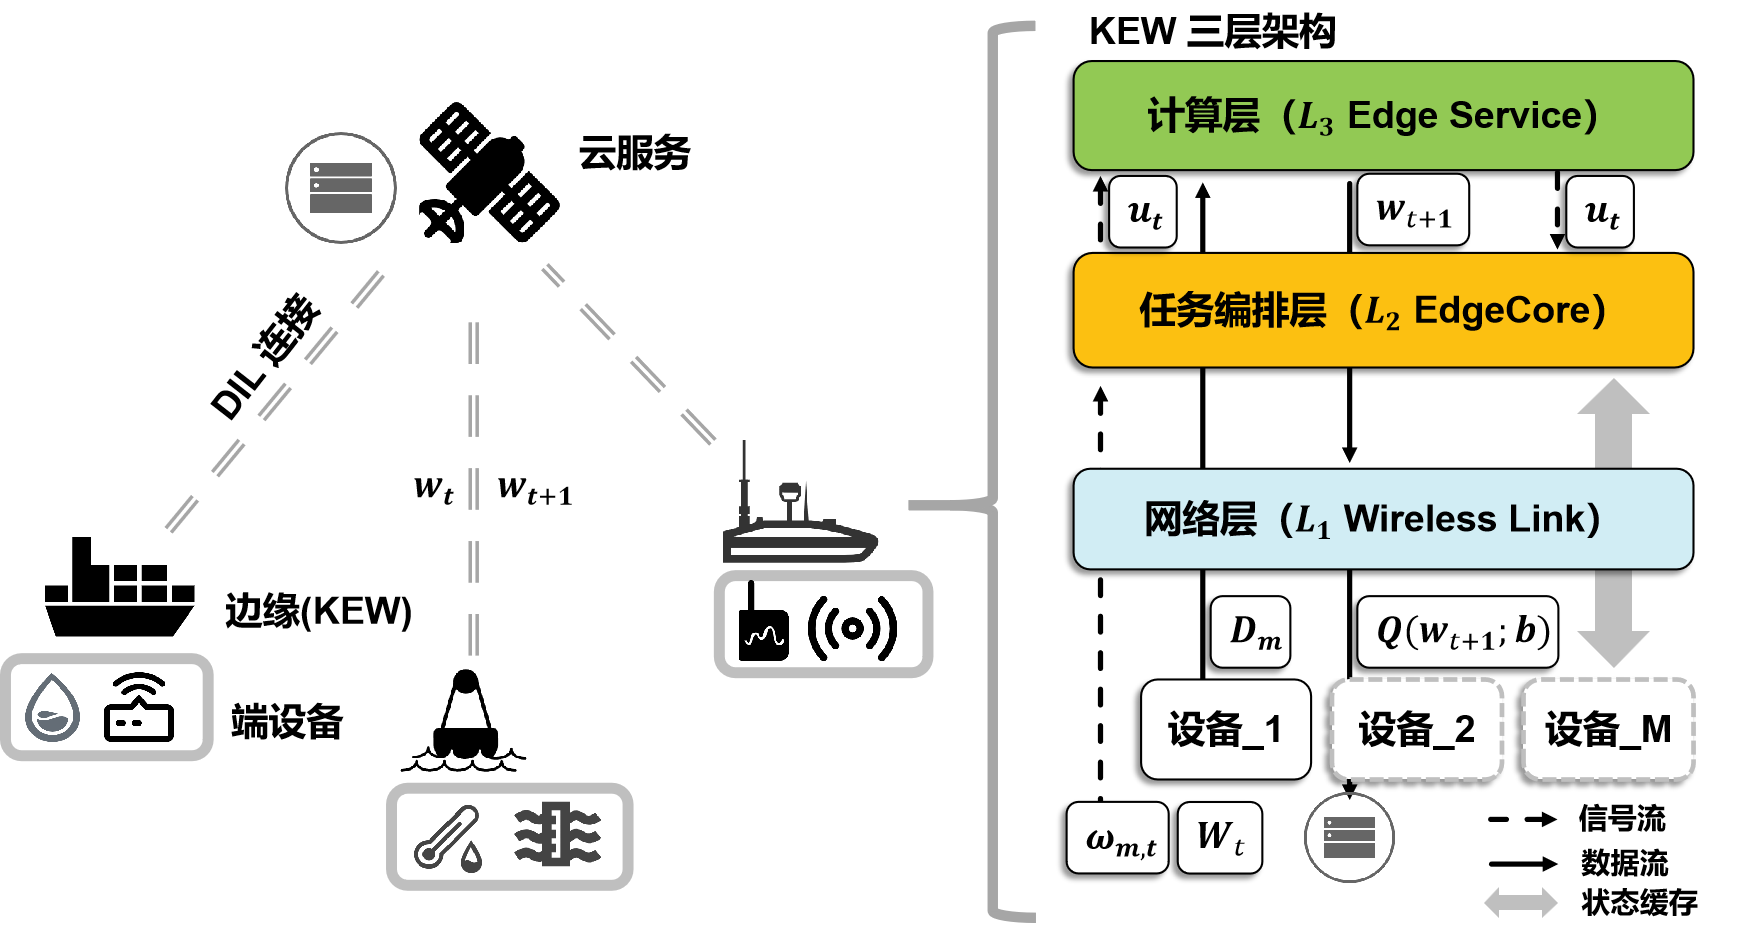
\includegraphics[width=0.80\textwidth]{kew_layer_flow.png}
\caption{Three-layer architecture and runtime workflow of the KEW platform. The architecture comprises the Compute Layer (Edge Service), Orchestration Layer (EdgeCore), and Network Layer (Wireless Link). Dashed arrows denote control and state signal flows, while solid arrows represent the flow of model parameters and task data across layers. The gray bidirectional arrow indicates the disconnection autonomy mechanism for policy caching during DIL conditions.}
\label{fig:kew_layer_flow}
\end{figure*}

\subsection{System Sensing Interface}
To establish a mathematical mapping between physical-layer environmental fluctuations and upper-layer algorithm decisions, KEW defines a standardized \textbf{system sensing interface} comprising observable and controllable variables.

\subsubsection{Observable Variables}
The state vector collected by the network layer and reported to the orchestration layer for client $m$ at round $t$ is defined as
\begin{equation}
    \boldsymbol{\omega}_{m,t} = \big[ R_{\text{down},m}(t), R_{\text{up},m}(t), \mathrm{RTT}_{m}(t), f_{m}(t), E_{m}(t) \big],
    \label{eq:omega}
\end{equation}
where $R_{\text{down},m}(t)$ and $R_{\text{up},m}(t)$ denote downlink and uplink effective throughput in Mbps, estimated over a sliding window $\Delta T$. The term $\mathrm{RTT}_m(t)$ represents the round-trip time in milliseconds, $f_m(t)$ is the available compute frequency in Hz, and $E_m(t)$ is the remaining energy budget in Joules. These variables serve as inputs for SA-FLQ algorithm decisions, reflecting the current link and node system state.

The orchestration layer determines the control vector $\mathbf{u}_t$ for each round. This vector includes the participating client set $\mathcal{S}_t \subseteq \mathcal{M}$, the number of local training epochs $I_{\text{loc},t}$, the round deadline $\tau_t$, and the quantization bitwidths $b_{\text{down}}(t)$ and $b_{\text{up}}(t)$ for downlink and uplink directions, expressed in bits per element.

\subsection{Delay and Energy Models}
Under DIL maritime conditions, the per-round training latency $T_{\text{round}}(t)$ comprises downlink broadcast, local computation, and uplink transmission, constrained by the slowest client (straggler):
\begin{equation}
    T_{\text{round}}(t) = \max_{m \in \mathcal{S}_t} \left\{ T_{\text{down},m}(t) + T_{\text{cmp},m}(t) + T_{\text{up},m}(t) \right\} + T_{\text{agg}},
    \label{eq:t_round}
\end{equation}
where $T_{\text{agg}}$ is the server-side aggregation time (typically negligible). The component latencies are
\begin{align}
    T_{\text{down},m}(t) &= \frac{D_{\text{model}} \cdot b_{\text{down}}(t)}{R_{\text{down},m}(t)}, \label{eq:t_down} \\
    T_{\text{cmp},m}(t) &= \frac{I_{\text{loc},t} \cdot n_m \cdot C_{\text{comp}}}{f_m(t)}, \label{eq:t_cmp} \\
    T_{\text{up},m}(t) &= \frac{D_{\text{grad}} \cdot b_{\text{up}}(t)}{R_{\text{up},m}(t)}, \label{eq:t_up}
\end{align}
where $D_{\text{model}}$ is the model parameter count, $n_m = |\mathcal{D}_m|$ is the local sample count, and $C_{\text{comp}}$ is the per-sample computation complexity measured in cycles per sample.

The total energy consumption of client $m$ at round $t$ includes computation and communication costs:
\begin{equation}
    E^{\text{total}}_m(t) = \kappa f_m^2(t) \cdot T_{\text{cmp},m}(t) + P_{\text{tx}} \cdot T_{\text{up},m}(t),
    \label{eq:energy}
\end{equation}
where $\kappa$ is the chip energy efficiency coefficient and $P_{\text{tx}}$ is the transmission power.

\subsection{Federated Learning Objective}
The goal of federated learning is to minimize the global loss function
\begin{equation}
    \min_{\mathbf{w}} F(\mathbf{w}) = \sum_{m=1}^{M} \frac{n_m}{n} F_m(\mathbf{w}),
    \label{eq:fl_obj}
\end{equation}
where $F_m(\mathbf{w}) = \frac{1}{n_m} \sum_{i \in \mathcal{D}_m} f_i(\mathbf{w})$ is the local loss function of client $m$.

\subsection{Constrained Optimization Formulation}
The core challenge in maritime edge federated learning is to minimize the global convergence error while satisfying strict latency and energy constraints by adjusting the control vector $\mathbf{u}_t$. This is formulated as a constrained optimization problem:
\begin{align}
    \min_{\mathbf{u}_t} \quad & \mathbb{E}\big[F(\mathbf{w}_{t+1})\big] \label{eq:opt_obj} \\
    \text{s.t.} \quad 
    & T_{\text{round}}(t) \leq \tau_t, \nonumber \\
    & E^{\text{total}}_m(t) \leq E_m(t), \quad \forall m \in \mathcal{S}_t, \nonumber \\
    & b_{\text{down}}(t), b_{\text{up}}(t) \in \{1, 2, 4, 8\}. \nonumber
\end{align}

This formulation reveals the \textbf{communication-computation-accuracy tradeoff}: reducing quantization bitwidths $b_{\text{down}}(t)$ and $b_{\text{up}}(t)$ significantly decreases communication latency, enabling the deadline constraint $\tau_t$ to be satisfied, but introduces quantization noise that may degrade model accuracy $F(\mathbf{w})$. The SA-FLQ algorithm presented in Section~\ref{sec:method} addresses this tradeoff through system-aware adaptive orchestration.

% ============================================================
%                    IV. METHODOLOGY
% ============================================================
\section{SA-FLQ Algorithm}
\label{sec:method}

This section presents the SA-FLQ (System-Aware Federated Low-bitwidth Quantization) algorithm. We first describe the framework overview, then detail the quantization strategies, and finally present the four-phase algorithm with adaptive bit selection.

\subsection{Framework Overview}
The proposed SA-FLQ framework is illustrated in Fig.~\ref{fig:flq_fed}. SA-FLQ integrates system-state sensing with adaptive quantization control through a closed-loop mechanism. Unlike conventional quantization methods that apply fixed compression, SA-FLQ dynamically adjusts quantization bitwidths based on real-time observable variables $\boldsymbol{\omega}_{m,t}$ collected from the KEW platform.

\begin{figure}[!t]
\centering
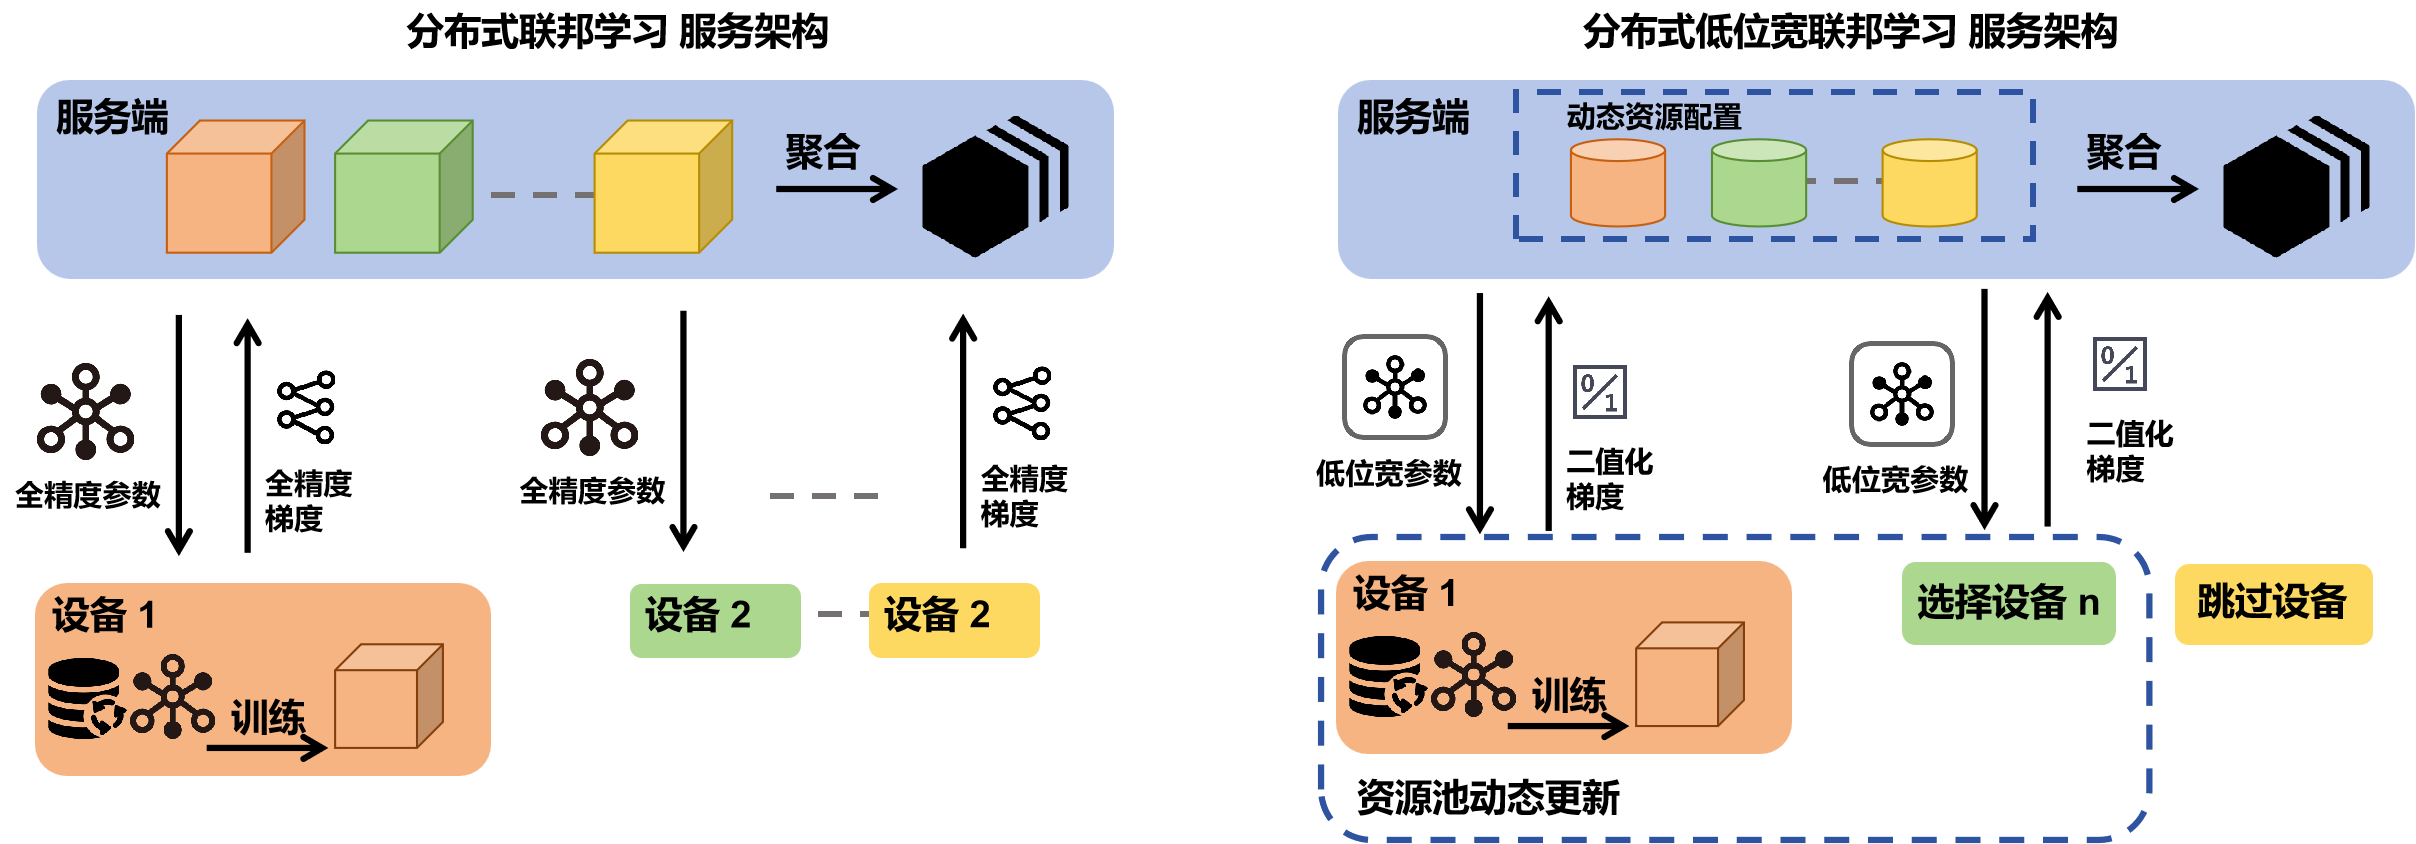
\includegraphics[width=0.9\columnwidth]{flq_fed.png}
\caption{Overview of the SA-FLQ framework. The system operates through a sense-decide-execute-writeback closed loop, where quantization strategies are dynamically adjusted based on real-time system state feedback from the KEW platform.}
\label{fig:flq_fed}
\end{figure}

\subsection{Per-Tensor Relative Quantization}
We introduce a per-tensor relative quantization strategy that quantizes gradient differences rather than absolute values. Given the gradient vector $\mathbf{g}^{(t)}$ at round $t$ and a reference vector $\mathbf{g}^{\text{ref}}$, the quantization is performed on the difference
\begin{equation}
    \Delta\mathbf{g}^{(t)} = \mathbf{g}^{(t)} - \mathbf{g}^{\text{ref}}.
\end{equation}

For symmetric $b$-bit quantization with $L = 2^{b-1} - 1$ levels, the quantization function is
\begin{equation}
    Q_b(x) = \text{sign}(x) \cdot \min\left(\left\lfloor \frac{|x|}{s} + 0.5 \right\rfloor, L\right),
\end{equation}
where $s = \frac{\max(|\Delta\mathbf{g}|)}{L}$ is the quantization scale.

The stochastic rounding variant adds randomness to enable unbiased estimation
\begin{equation}
    Q_b^{\text{stoch}}(x) = \text{sign}(x) \cdot \left\lfloor \frac{|x|}{s} + \xi \right\rfloor,
\end{equation}
where $\xi \sim \text{Uniform}(0, 1)$.

\subsection{Adaptive Bit Selection Policy}
A key innovation of SA-FLQ is the adaptive selection of quantization bitwidths based on system state. Given the observable variables $\boldsymbol{\omega}_{m,t}$ and training progress, we define the bit selection policy:
\begin{equation}
    (b_{\text{down}}(t), b_{\text{up}}(t)) = 
    \begin{cases}
        (b_{\max}, b_{\max}), & \|\bar{\mathbf{g}}_{t-1}\| > \delta_{\text{grad}} \\
        (b_{\min}, b_{\min}), & \mathrm{RTT}(t) > \delta_{\text{rtt}} \\
        (b_{\text{mid}}, b_{\text{mid}}), & \text{otherwise}
    \end{cases}
    \label{eq:bit_policy}
\end{equation}
where $\delta_{\text{grad}}$ and $\delta_{\text{rtt}}$ are threshold parameters, and $\bar{\mathbf{g}}_{t-1}$ is the aggregated gradient from the previous round. Since the exact global gradient $\nabla F(\mathbf{w}_t)$ is unavailable at the server without accessing all client data, we use the previous round's aggregated update as a practical proxy. This policy uses higher precision during early training when gradient magnitudes are large, and switches to aggressive compression when link quality degrades as indicated by high RTT values.

\subsection{SA-FLQ Algorithm}
The complete SA-FLQ algorithm is presented in Algorithm~\ref{alg:saflq}, structured into four explicit phases that embody the sense-decide-execute-writeback closed loop.

\begin{algorithm}[!t]
\caption{SA-FLQ: System-Aware Federated Low-bitwidth Quantization}
\label{alg:saflq}
\begin{algorithmic}[1]
\STATE \textbf{Input:} Initial model $\mathbf{w}^{(0)}$, learning rate $\eta$, max rounds $T$, client set $\mathcal{M}$, constraints $\tau_{\max}, E_{\min}$
\STATE \textbf{Output:} Trained global model $\mathbf{w}^{(T)}$
\FOR{$t = 0, 1, \ldots, T-1$}
    \STATE \textbf{// Phase 1: Sense \& Decide}
    \FOR{each client $m \in \mathcal{M}$ in parallel}
        \STATE Network layer collects $\boldsymbol{\omega}_{m,t} = [R_{\text{up}}, R_{\text{down}}, \mathrm{RTT}, E, f]$
        \STATE Report $\boldsymbol{\omega}_{m,t}$ to orchestration layer
    \ENDFOR
    \STATE Compute device scores: $\pi_{m,t} = R_{\text{up},m} \cdot \frac{E_m}{E_{\max}} \cdot \frac{n_m}{n}$
    \STATE Select participating set: $\mathcal{S}_t = \text{TopK}(\{\pi_{m,t}\}_m)$
    \STATE Determine bitwidths $(b_{\text{down}}, b_{\text{up}})$ via Eq.~\eqref{eq:bit_policy}
    \STATE Generate control vector: $\mathbf{u}_t = (\mathcal{S}_t, b_{\text{down}}, b_{\text{up}}, I_{\text{loc},t})$
    
    \STATE \textbf{// Phase 2: Broadcast}
    \STATE Quantize global model: $\hat{\mathbf{w}}_t = Q_{b_{\text{down}}}(\mathbf{w}_t)$
    \STATE Broadcast $\hat{\mathbf{w}}_t$ and $\mathbf{u}_t$ to clients in $\mathcal{S}_t$
    
    \STATE \textbf{// Phase 3: Collaborative Execution}
    \FOR{each client $m \in \mathcal{S}_t$ in parallel}
        \STATE Load local data $\mathcal{D}_m$ and model $\hat{\mathbf{w}}_t$
        \FOR{$k = 0, 1, \ldots, I_{\text{loc},t}-1$}
            \STATE Sample minibatch $\mathcal{B}_m$ from $\mathcal{D}_m$
            \STATE $\mathbf{g}_m^{(k)} \leftarrow \nabla F_m(\mathbf{w}_m; \mathcal{B}_m)$
            \STATE $\mathbf{w}_m \leftarrow \mathbf{w}_m - \eta \mathbf{g}_m^{(k)}$
        \ENDFOR
        \STATE Compute update: $\Delta\mathbf{w}_m = \mathbf{w}^{(t)} - \mathbf{w}_m$
        \STATE Adaptive quantization: $\hat{\Delta}\mathbf{w}_m = Q_{b_{\text{up}}}(\Delta\mathbf{w}_m)$
        \STATE Upload $\hat{\Delta}\mathbf{w}_m$ via uplink DIL channel
    \ENDFOR
    
    \STATE \textbf{// Phase 4: Aggregation \& Writeback}
    \STATE Server dequantizes and aggregates:
    \STATE \quad $\bar{\mathbf{g}}_t = \frac{1}{\sum_{m \in \mathcal{S}_t} n_m} \sum_{m \in \mathcal{S}_t} n_m \cdot \text{Dequant}(\hat{\Delta}\mathbf{w}_m)$
    \STATE Update global model: $\mathbf{w}^{(t+1)} = \mathbf{w}^{(t)} - \eta_t \bar{\mathbf{g}}_t$
    \STATE Writeback: Record $T_{\text{round}}$, energy consumption, update statistics
\ENDFOR
\end{algorithmic}
\end{algorithm}

\textbf{In the Sense \& Decide phase}, the network layer continuously monitors DIL channel conditions and node states. It reports observable variables $\boldsymbol{\omega}_{m,t}$ to the orchestration layer. Based on these observations, the orchestrator computes device priority scores that consider uplink quality, remaining energy, and data contribution. High-scoring devices are selected for participation, and quantization bitwidths are determined adaptively based on the estimated global gradient from the previous round.

\textbf{In the Broadcast phase}, the server quantizes the global model using $b_{\text{down}}$ bits and transmits it alongside the control vector $\mathbf{u}_t$. Since satellite links are bandwidth-constrained, this low-bitwidth broadcasting strategy is crucial for reducing downlink latency.

\textbf{In the Collaborative Execution phase}, each participating client performs $I_{\text{loc}}$ epochs of local training on its private data. The resulting model updates are quantized using $b_{\text{up}}$ bits before transmission. The network layer applies adaptive quantization based on current link conditions.

\textbf{In the Aggregation \& Writeback phase}, the server receives and dequantizes updates from all participants, performs weighted aggregation, and updates the global model. Key metrics such as round latency, energy consumption, and accuracy are written back to the system for closed-loop optimization in subsequent rounds.



\subsection{Convergence Analysis}
We analyze the convergence properties of SA-FLQ under standard assumptions commonly used in federated learning analysis.

\textbf{Assumption 1} (L-Smoothness): The loss function $F$ is $L$-smooth, i.e., for all $\mathbf{w}, \mathbf{v}$
\begin{equation}
    \|\nabla F(\mathbf{w}) - \nabla F(\mathbf{v})\| \leq L\|\mathbf{w} - \mathbf{v}\|.
\end{equation}

\textbf{Assumption 2} (Bounded Variance): The stochastic gradient has bounded variance
\begin{equation}
    \mathbb{E}\|\nabla F_m(\mathbf{w}; \xi) - \nabla F_m(\mathbf{w})\|^2 \leq \sigma^2,
\end{equation}
where $\xi$ represents random sampling.

\textbf{Assumption 3} (Bounded Gradient Dissimilarity): The gradient dissimilarity across clients is bounded
\begin{equation}
    \frac{1}{M}\sum_{m=1}^{M}\|\nabla F_m(\mathbf{w}) - \nabla F(\mathbf{w})\|^2 \leq \delta^2.
\end{equation}

We first establish the quantization error bound.

\textbf{Lemma 1} (Quantization Error Bound): For symmetric $b$-bit stochastic quantization with scale $s = \frac{\max(|\mathbf{g}|)}{2^{b-1}-1}$, the quantization error satisfies
\begin{equation}
    \mathbb{E}\|Q_b(\mathbf{g}) - \mathbf{g}\|^2 \leq \frac{d \cdot s^2}{4} = \frac{d \cdot \|\mathbf{g}\|_\infty^2}{4(2^{b-1}-1)^2},
\end{equation}
where $d$ is the dimension of the gradient vector.

\textit{Proof of Lemma 1:} For each element $g_i$, the stochastic quantization ensures $\mathbb{E}[Q_b(g_i)] = g_i$ (unbiasedness). The variance of quantization is bounded by $\mathbb{E}[(Q_b(g_i) - g_i)^2] \leq s^2/4$ since the maximum rounding error is $s/2$. Summing over all $d$ dimensions yields the bound. $\square$

\textbf{Theorem 1} (Convergence of SA-FLQ): Under Assumptions 1-3, let $\eta = \frac{1}{L\sqrt{KT}}$ be the learning rate, $K$ be the local update steps, and $b$ be the quantization bits. After $T$ communication rounds, SA-FLQ satisfies
\begin{equation}
\begin{split}
    \frac{1}{T}\sum_{t=0}^{T-1}\mathbb{E}\|\nabla F(\mathbf{w}^{(t)})\|^2 \leq & \underbrace{\frac{2L(F(\mathbf{w}^{(0)}) - F^*)}{\sqrt{KT}}}_{\text{optimization error}} \\
    & + \underbrace{\frac{2\sigma^2}{M\sqrt{KT}}}_{\text{variance error}} + \underbrace{\frac{2K\delta^2}{\sqrt{KT}}}_{\text{heterogeneity error}} \\
    & + \underbrace{\frac{2\epsilon_q^2}{T}}_{\text{quantization error}},
\end{split}
\end{equation}
where $F^* = \min_{\mathbf{w}} F(\mathbf{w})$ is the optimal value, and $\epsilon_q^2 = \frac{d \cdot G^2}{4(2^{b-1}-1)^2}$ with $G = \max_t \|\mathbf{g}^{(t)}\|_\infty$.

\textbf{Corollary 1} (Communication-Accuracy Tradeoff): The quantization error term $\epsilon_q^2$ decreases exponentially with $b$. Specifically, doubling the number of bits reduces the quantization error by approximately $4\times$
\begin{equation}
    \frac{\epsilon_q^2(b)}{\epsilon_q^2(2b)} \approx 4^b.
\end{equation}

This corollary explains the empirical observation that moderate quantization (4-8 bits) achieves near full-precision accuracy, as the quantization error becomes negligible compared to other error sources.

% ============================================================
%                    V. EXPERIMENTS
% ============================================================
\section{Experiments}
\label{sec:experiments}

\subsection{Experimental Settings}

\subsubsection{Datasets}
We evaluate SA-FLQ on three datasets with increasing complexity:

\textbf{MNIST}: A handwritten digit recognition dataset with 60,000 training and 10,000 test images of size $28 \times 28$ grayscale.

\textbf{Fashion-MNIST}: A fashion product classification dataset with the same structure as MNIST but more challenging patterns.

\textbf{Oil Detection Dataset}: A real-world maritime oil spill detection dataset collected from aerial and satellite imagery of ocean surfaces containing 2,811 annotated images with bounding box labels for oil spill regions.

\subsubsection{Data Distribution}
To simulate realistic federated learning scenarios, we create non-IID data partitions using the Dirichlet distribution with concentration parameter $\alpha = 0.3$.

\subsubsection{Baselines}
We compare SA-FLQ with five baseline methods:

\textbf{FedAvg}: Standard federated averaging with full-precision communication.

\textbf{QSGD}: Quantized stochastic gradient descent with multiple bit-widths.

\textbf{SignSGD}: Extreme 1-bit quantization using only gradient signs.

\textbf{Top-K}: Gradient sparsification transmitting only top elements.

\textbf{LAQ}: Lazily aggregated quantized gradient innovation.

\subsubsection{Implementation Details}
For simulation experiments, we use a CNN with two convolutional layers and two fully connected layers (approximately 1.2M parameters). For oil detection, we employ YOLOv8n (approximately 3.2M parameters). All experiments use SGD optimizer with momentum 0.9 and weight decay $5 \times 10^{-4}$. The learning rate is initialized at 0.01 with cosine annealing schedule.

\subsection{Simulation Results}

\subsubsection{Convergence Analysis}
Fig.~\ref{fig:convergence} presents the convergence behavior of SA-FLQ compared to baseline methods on Fashion-MNIST with $M=10$ clients and non-IID distribution ($\alpha=0.3$).

\begin{figure}[!t]
\centering
\subfloat[Training loss convergence]{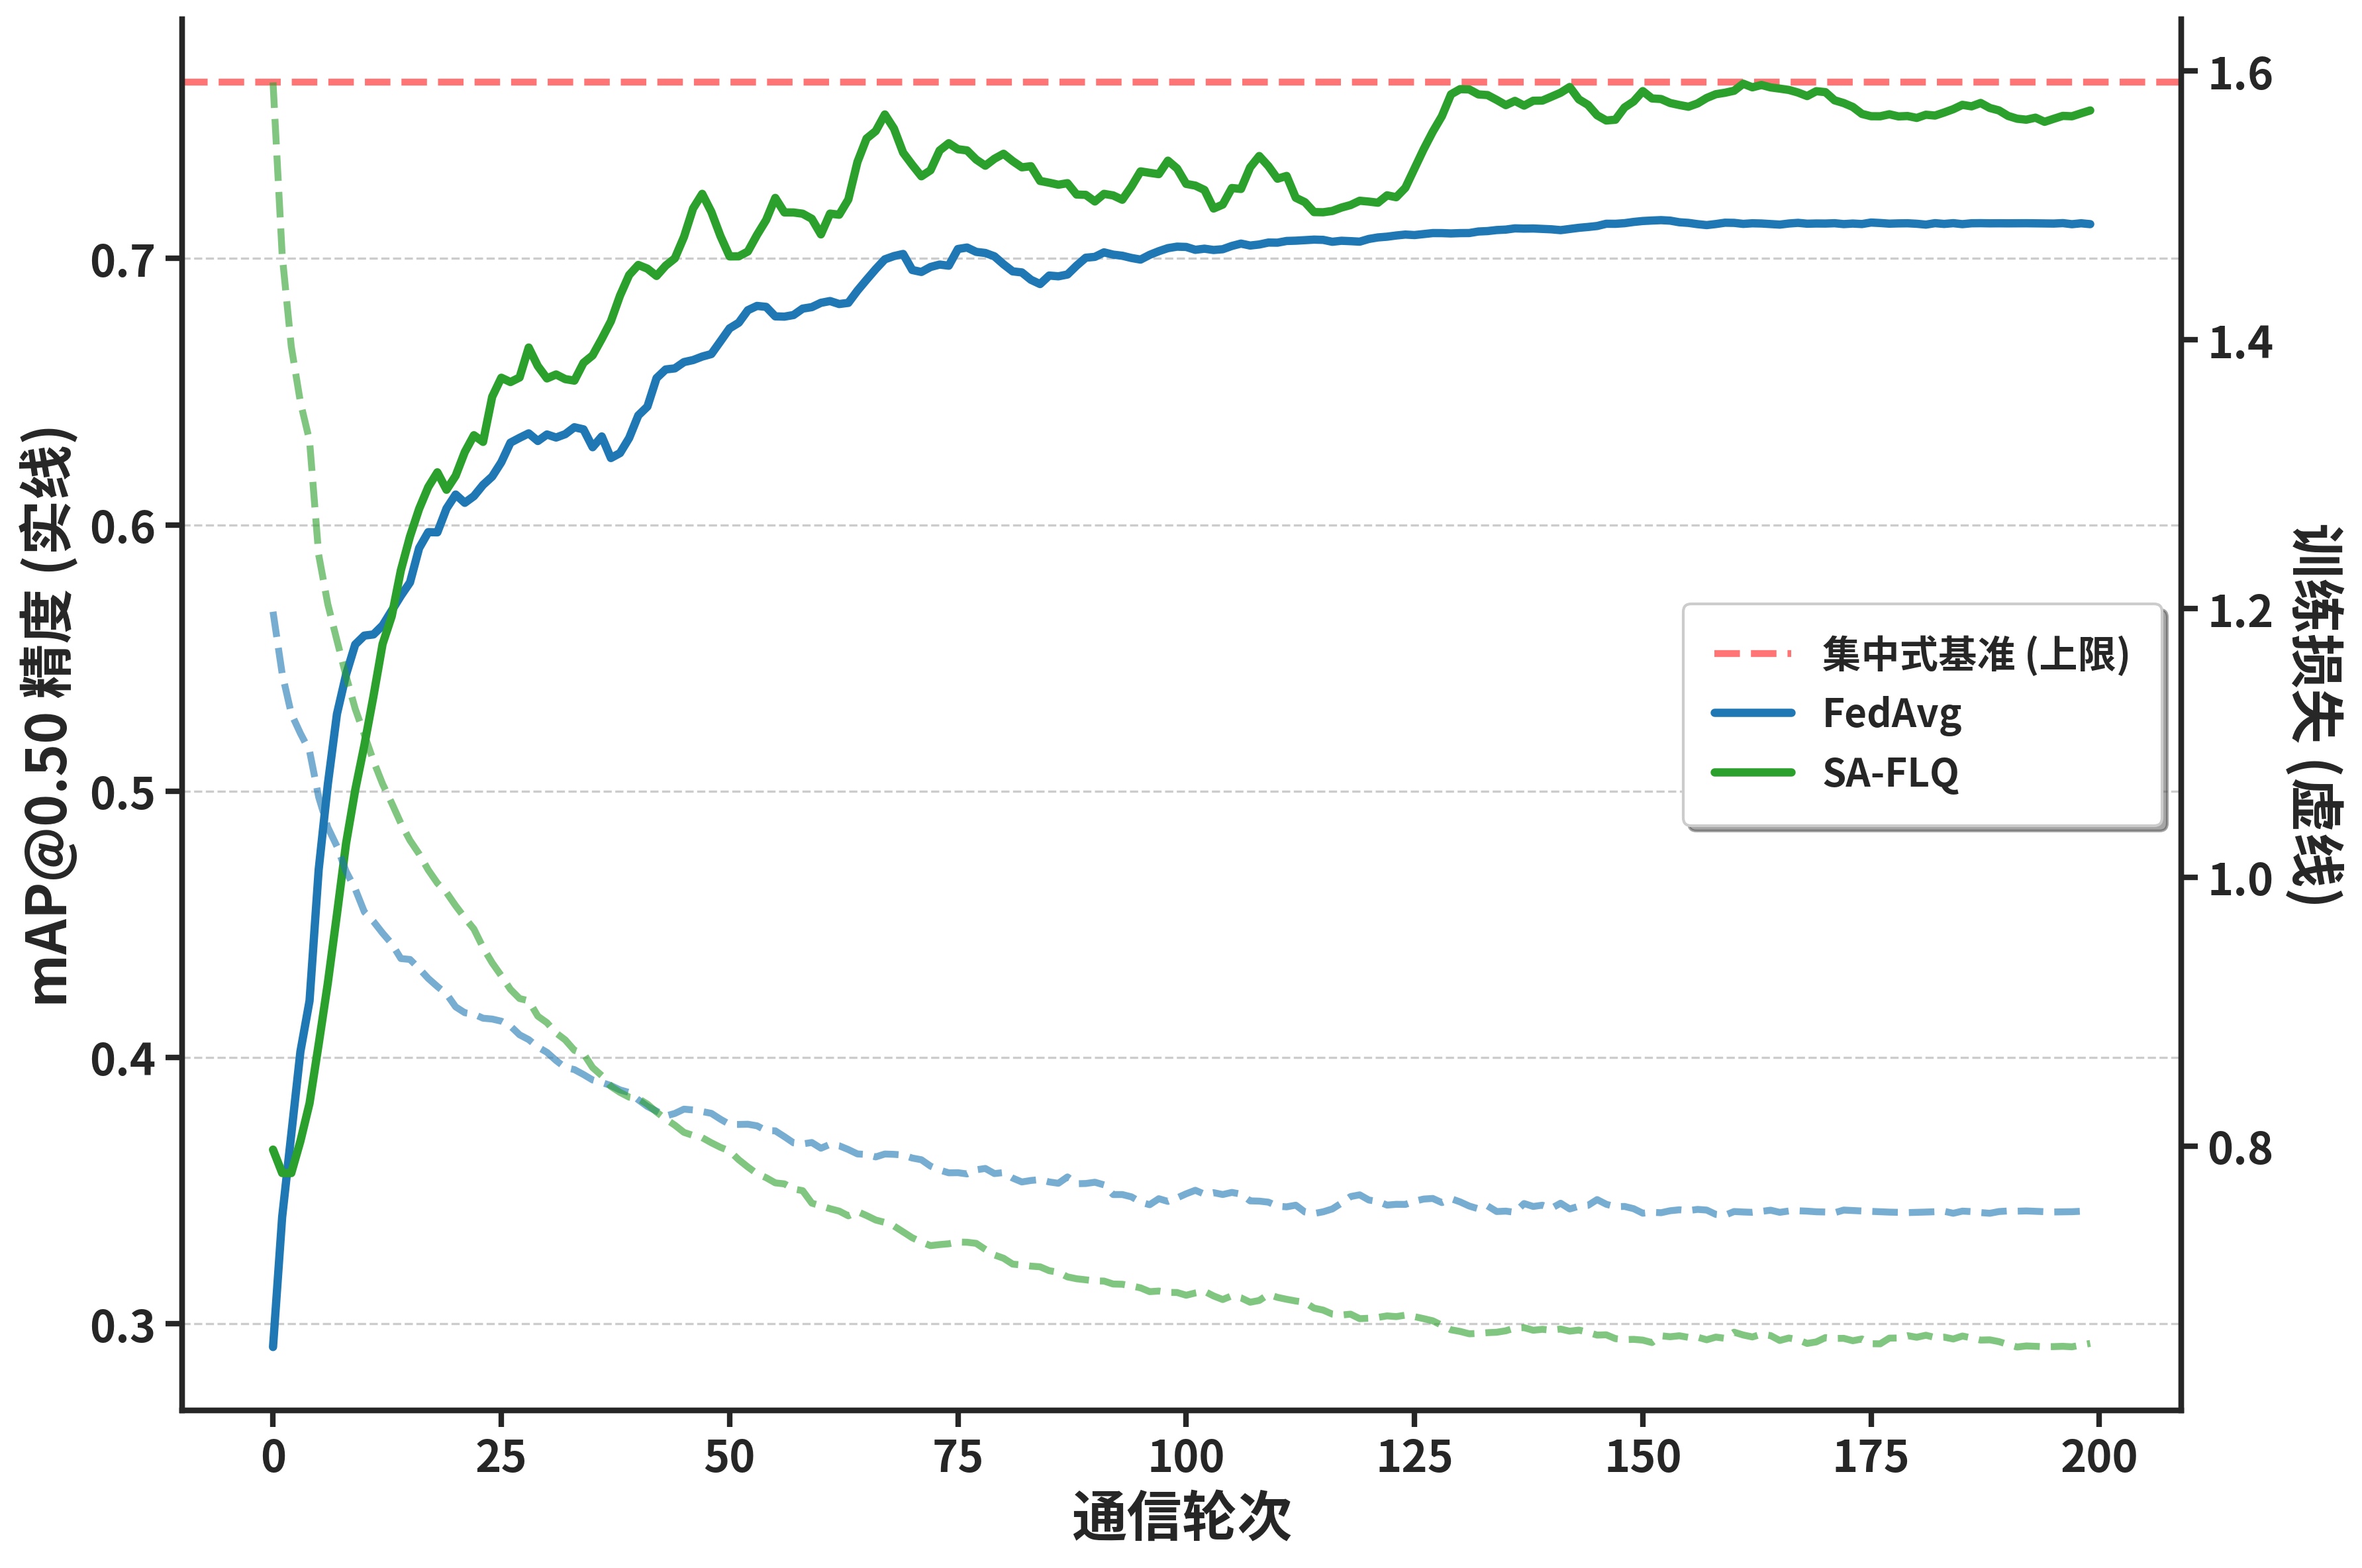
\includegraphics[width=0.45\columnwidth]{convergence_loss_cn.png}}
\hfil
\subfloat[Test accuracy convergence]{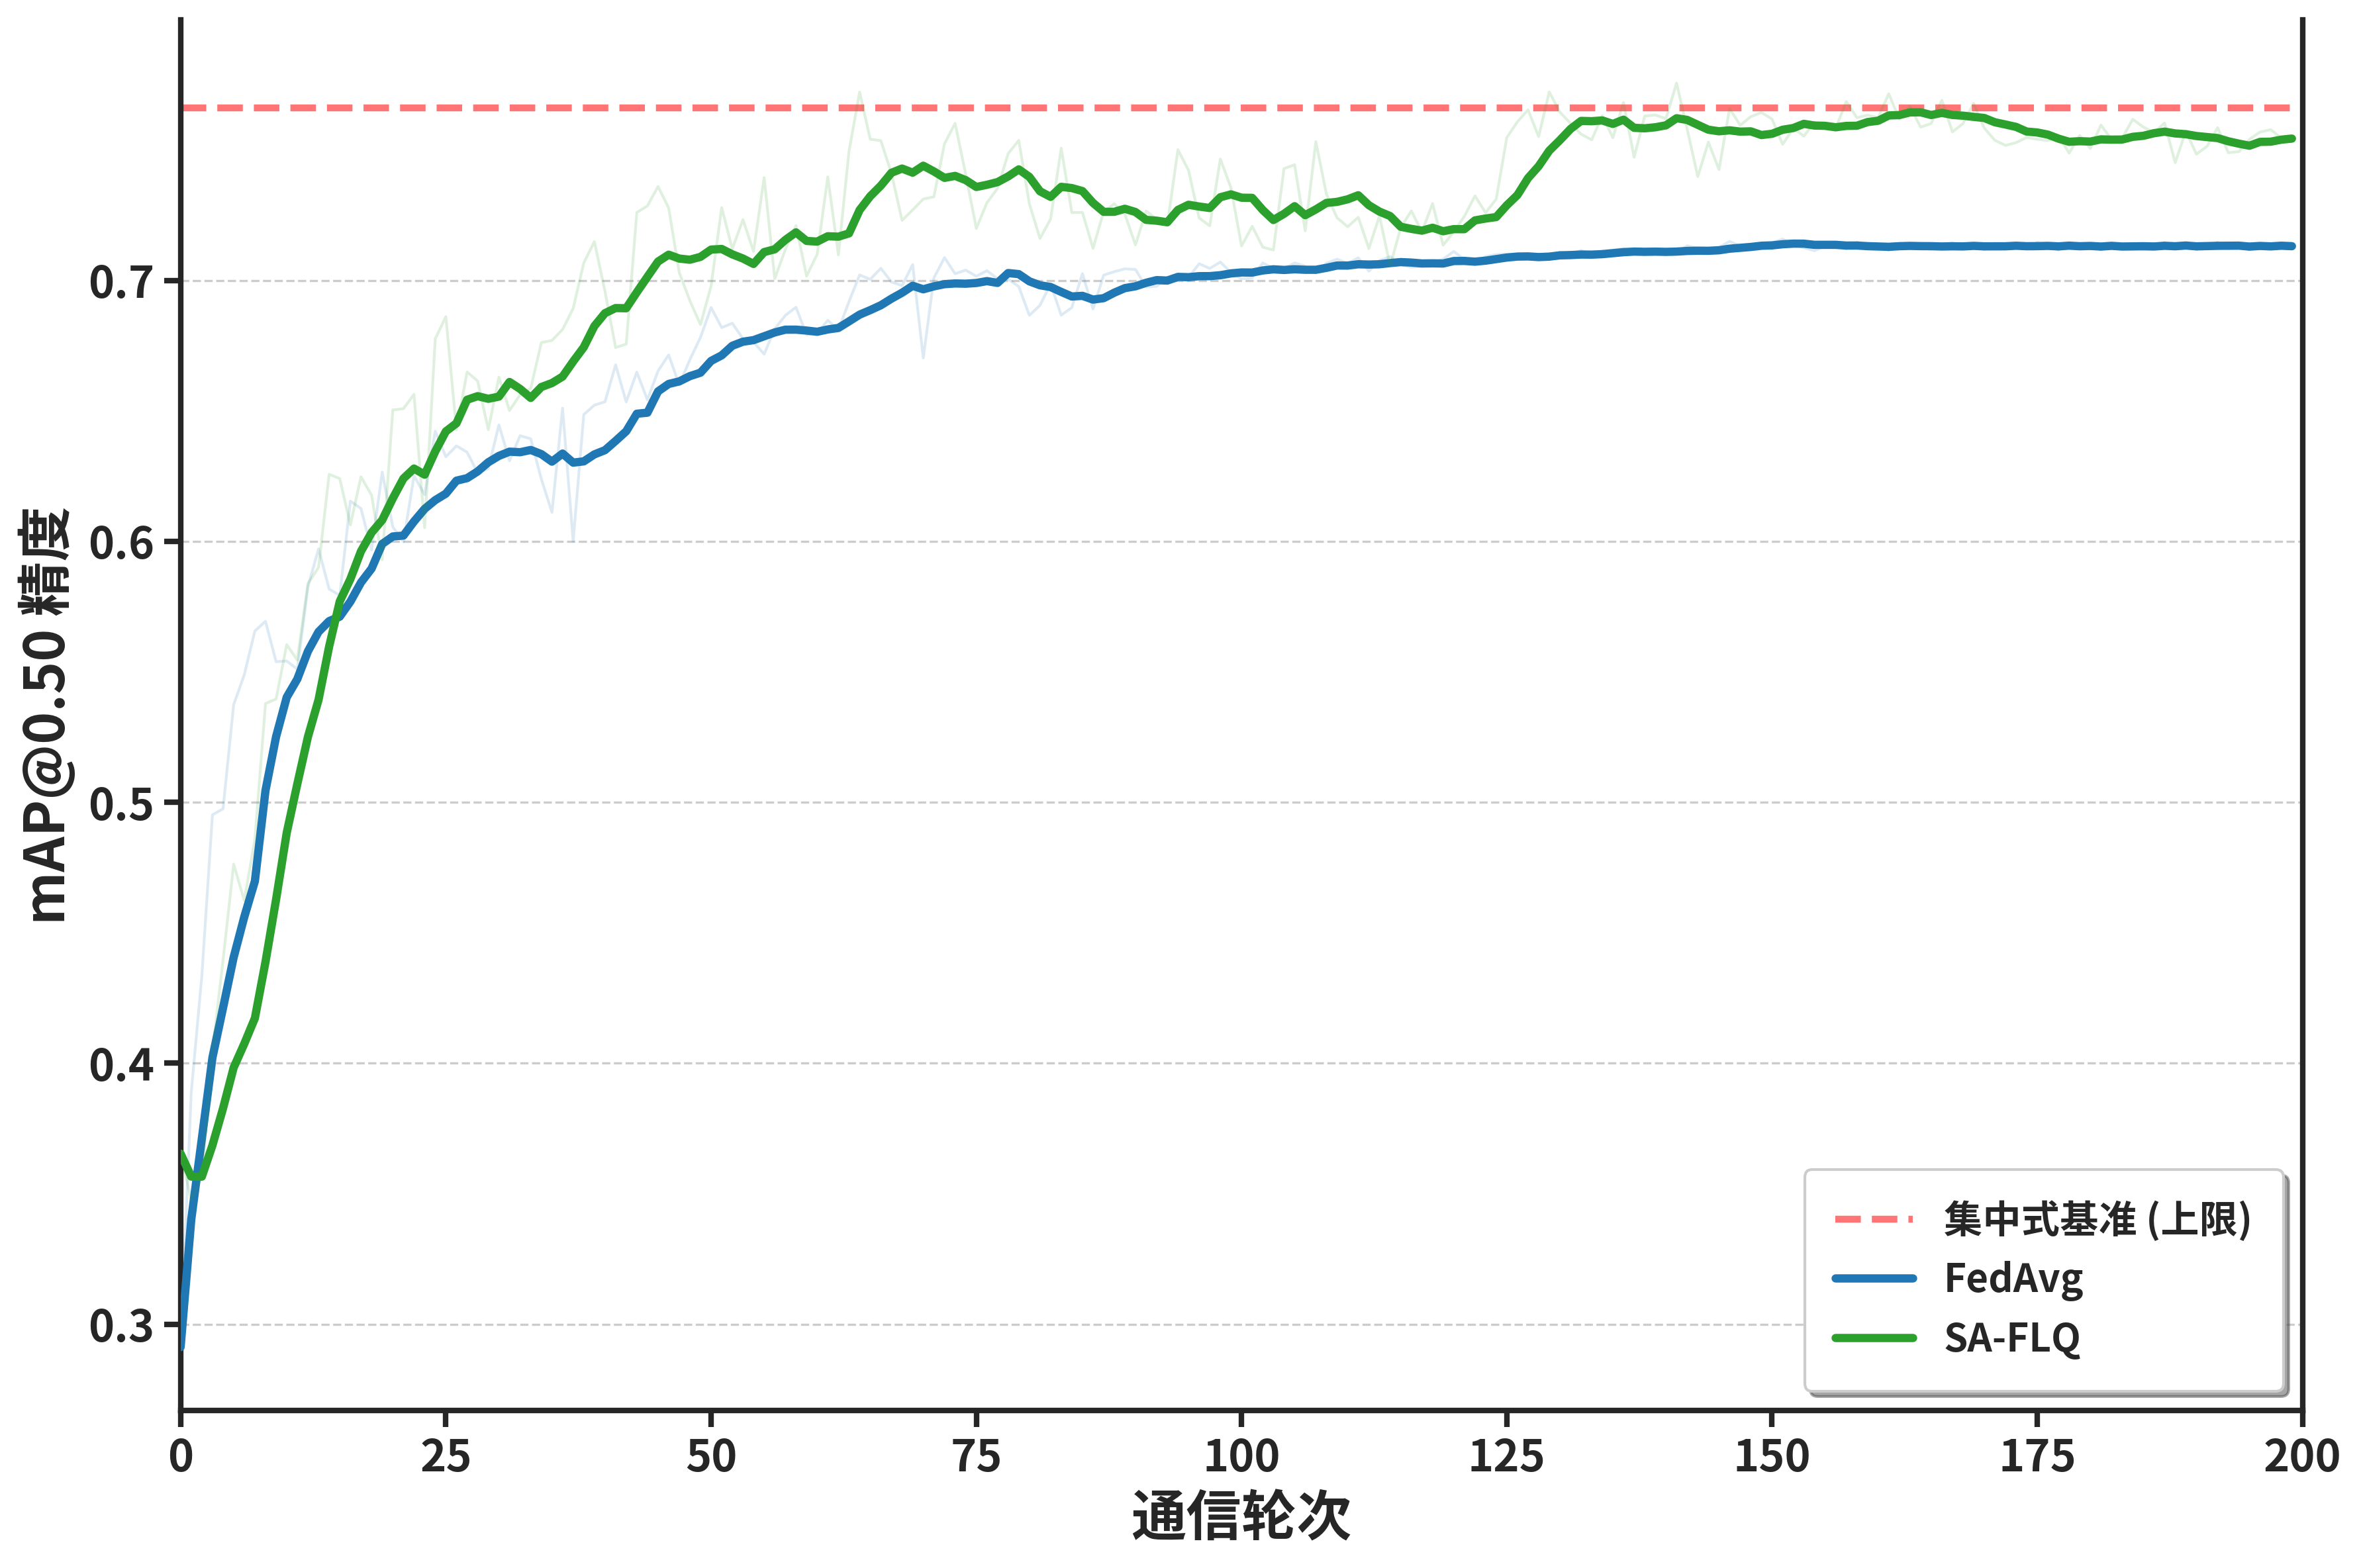
\includegraphics[width=0.45\columnwidth]{map_convergence_cn.png}}
\caption{Convergence analysis on Fashion-MNIST with $M=10$ clients. SA-FLQ achieves near full-precision performance with significant communication reduction.}
\label{fig:convergence}
\end{figure}

SA-FLQ with 8-bit quantization achieves convergence behavior nearly identical to full-precision FedAvg with final accuracy difference less than $0.3\%$. With 4-bit quantization, SA-FLQ reaches $97.8\%$ of full-precision accuracy while achieving $8\times$ compression.

\subsubsection{Quantization Bit-Width Comparison}
Fig.~\ref{fig:bit_comparison} shows the impact of different quantization bit-widths on model accuracy.

\begin{figure}[!t]
\centering

\includegraphics[width=0.9\columnwidth]{Fig2_fmnist.png}
\caption{Performance comparison under different quantization bit-widths on Fashion-MNIST. SA-FLQ consistently outperforms baselines across all configurations.}
\label{fig:bit_comparison}
\end{figure}

\subsection{Gradient Quantization Analysis}
To further explain why SA-FLQ maintains stable convergence under aggressive compression, Fig.~\ref{fig:gradient_quant} visualizes the binary gradient quantization process throughout training. The figure shows how continuous gradient values are forced into binary states $\{0, 1\}$ across communication rounds.

\begin{figure}[!t]
\centering
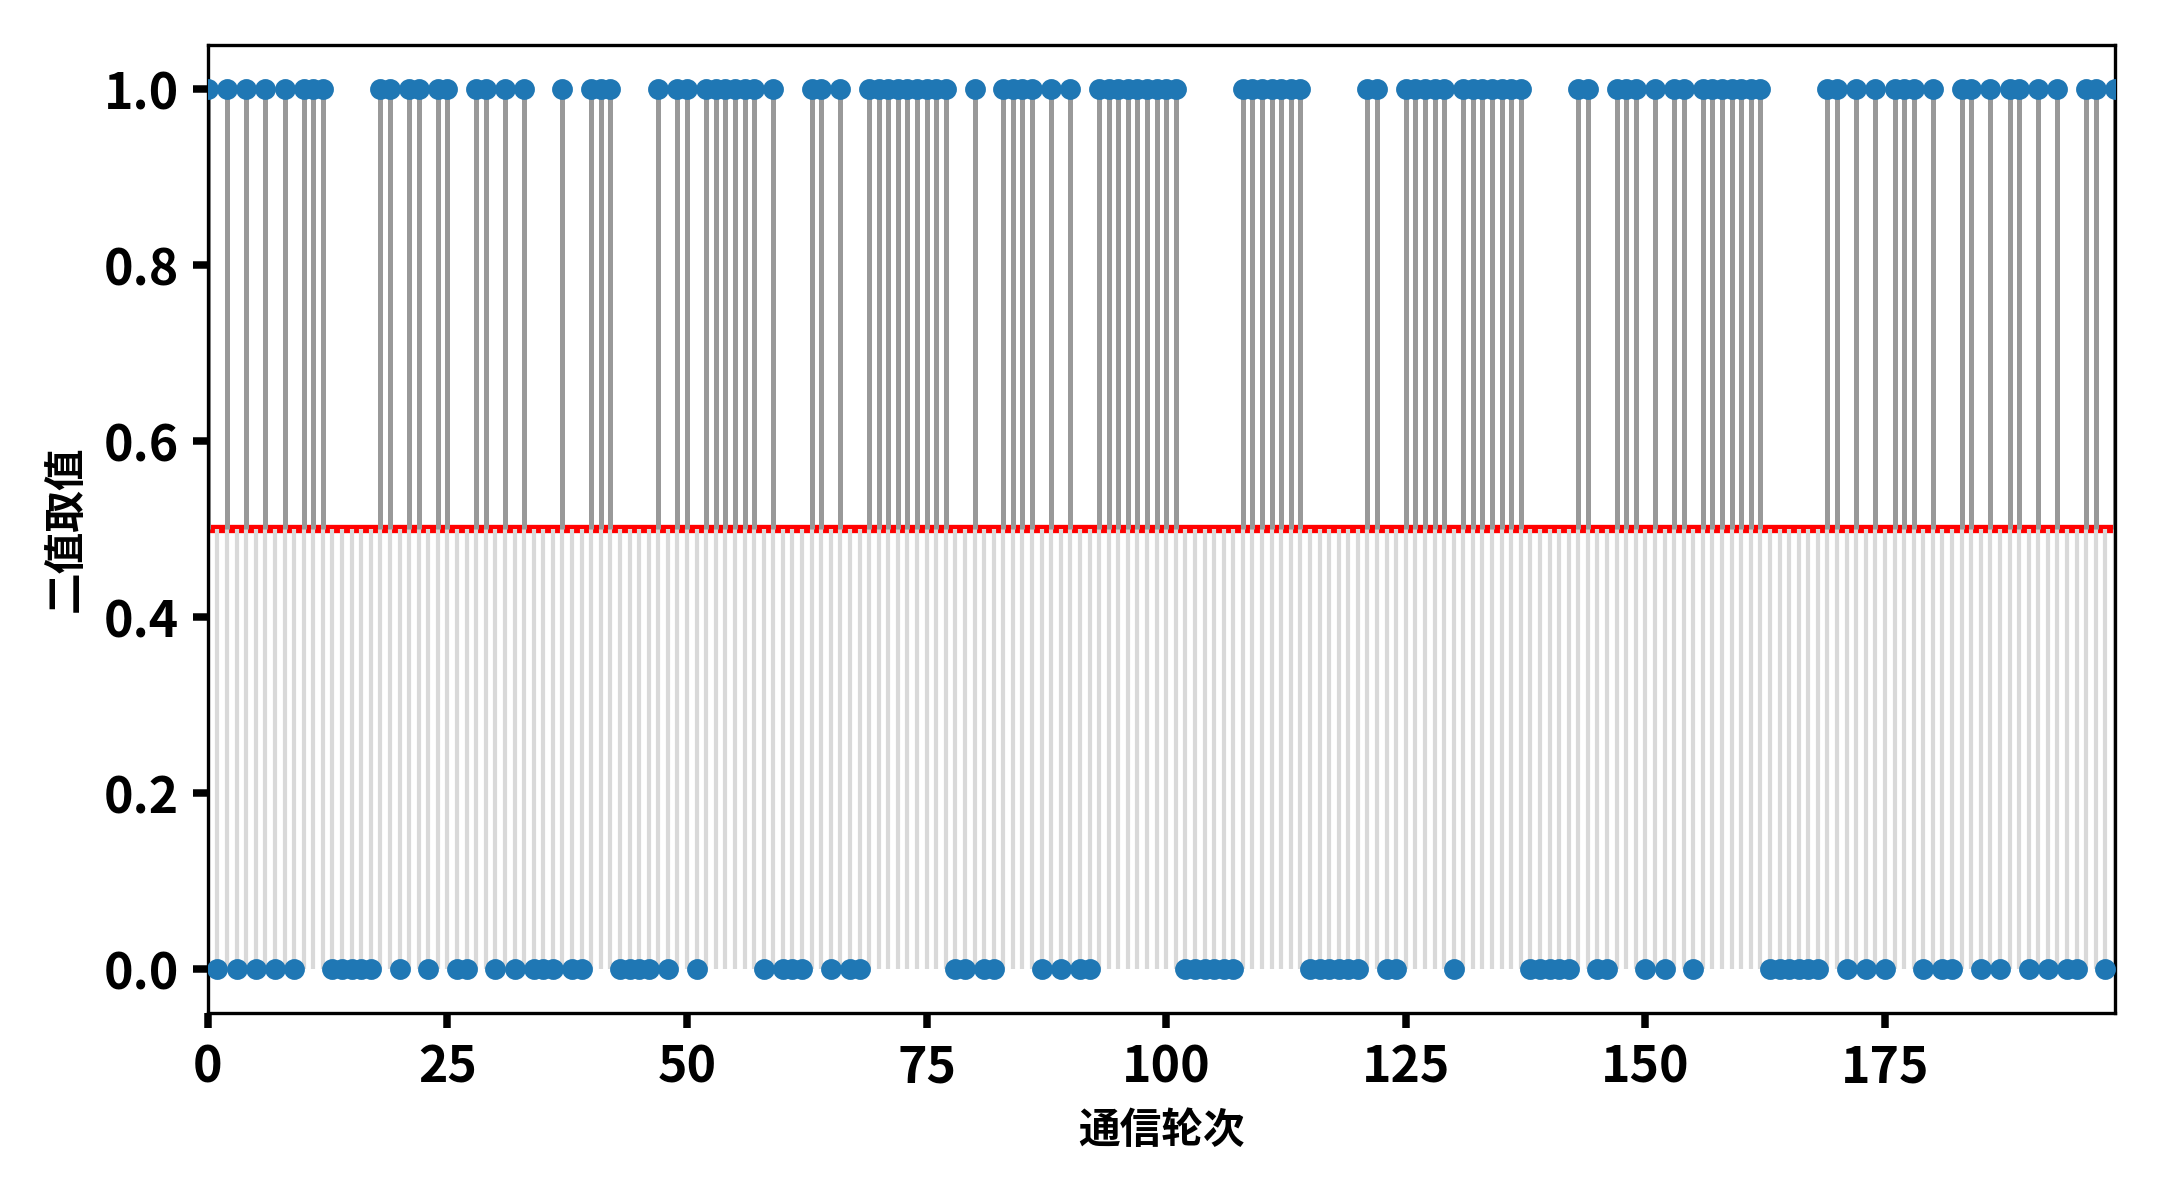
\includegraphics[width=0.9\columnwidth]{gradient_quantification.jpg}
\caption{Visualization of binary gradient quantization during SA-FLQ training. Blue dots show continuous gradient values mapped to binary states $\{0, 1\}$, with the red line ($y=0.5$) indicating the quantization threshold. Early training shows frequent transitions reflecting exploration, while later rounds exhibit stable block patterns indicating consistent descent directions.}
\label{fig:gradient_quant}
\end{figure}

Fig.~\ref{fig:k_parameter} compares gradient approximation performance under different quantization bitwidths. At $k=4$, quantized values show visible noise around true values with RMSE of 0.0138. At $k=8$, quantized values align tightly with true gradients, reducing RMSE to 0.0006, indicating near-lossless numerical fidelity.

\begin{figure}[!t]
\centering
\subfloat[$k=4$: RMSE = 0.0138]{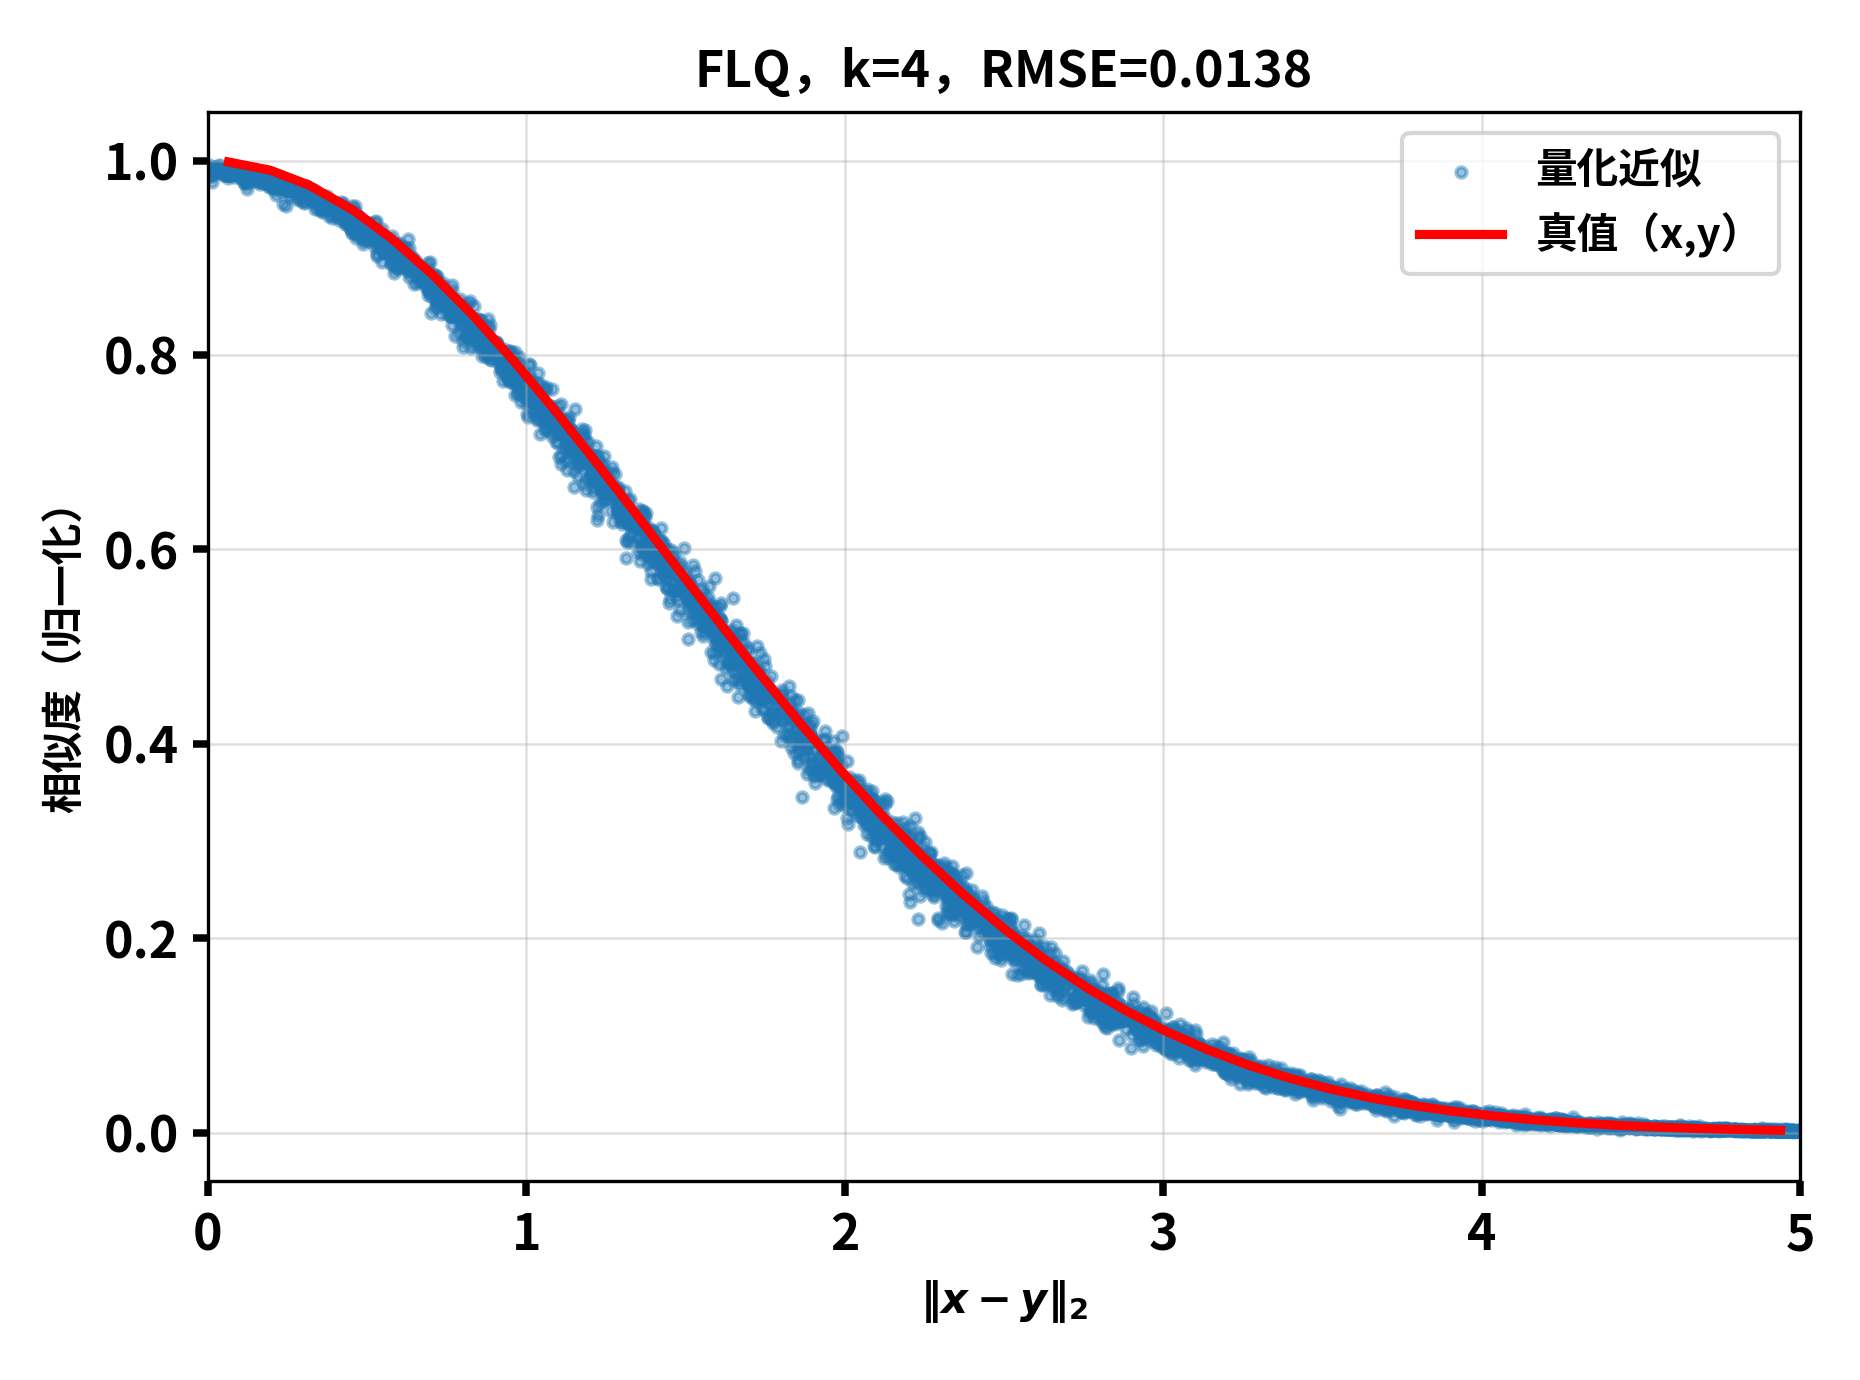
\includegraphics[width=0.48\columnwidth]{Fig4_k4_fmnist.png}}
\hfil
\subfloat[$k=8$: RMSE = 0.0006]{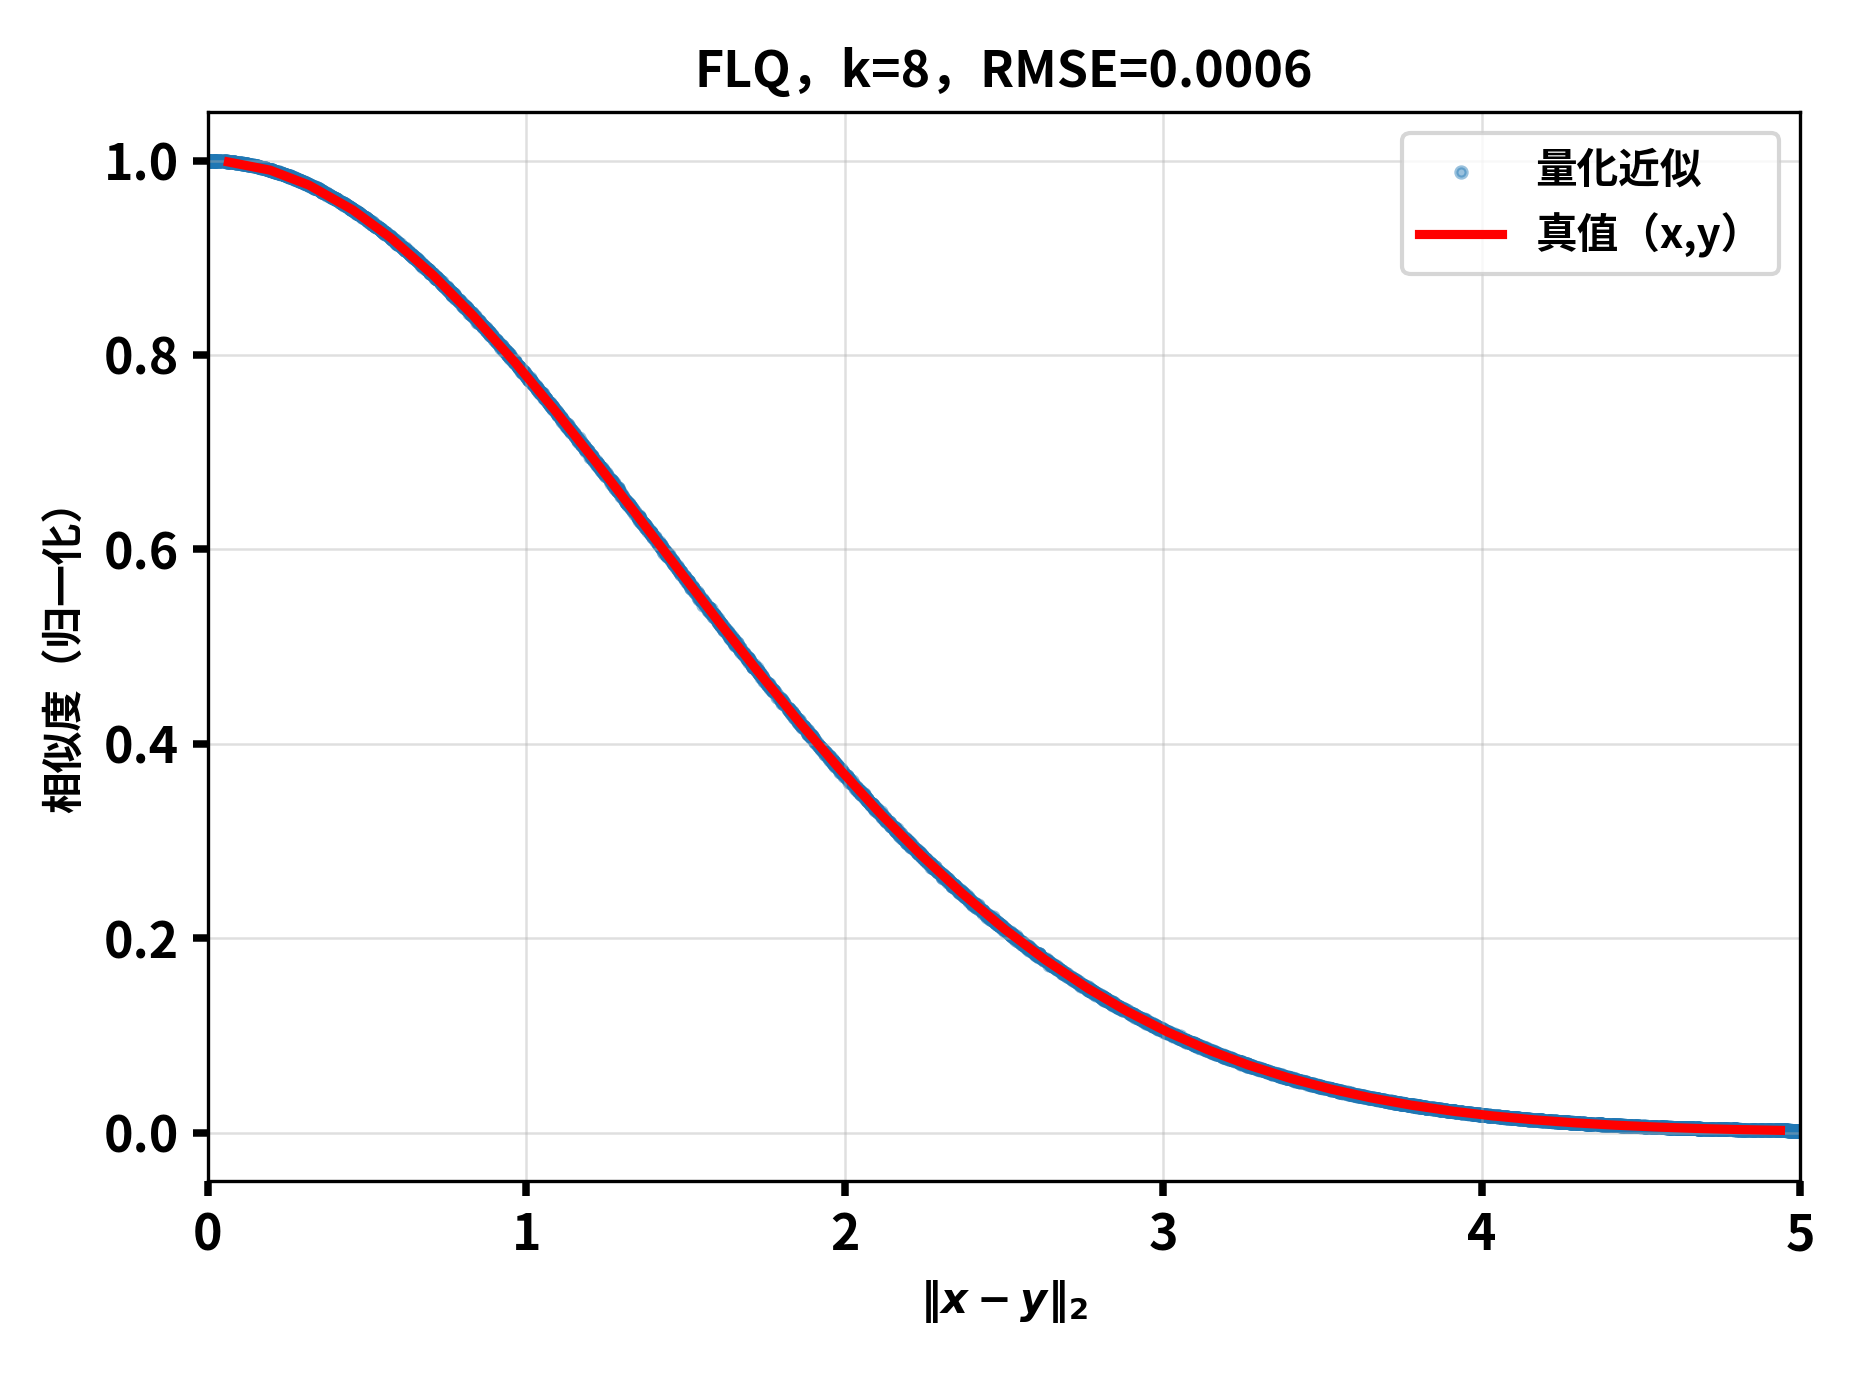
\includegraphics[width=0.48\columnwidth]{Fig4_k8_fmnist.png}}
\caption{Gradient approximation performance under different quantization bitwidths. At $k=4$, visible noise exists around true values. At $k=8$, quantized values closely match true gradients, demonstrating near-lossless fidelity while still achieving significant communication reduction.}
\label{fig:k_parameter}
\end{figure}

Based on our analysis, $k=4$ with adaptive bit selection provides an excellent balance, achieving $98\%$ of full-precision accuracy while reducing total communication by $8\times$.

\subsection{Real-World Deployment: Oil Spill Detection}
We deploy SA-FLQ on a testbed consisting of three NVIDIA Jetson Xavier NX edge devices simulating distributed maritime monitoring stations.

\subsubsection{Deployment Setup}
Each node uses an NVIDIA Jetson Xavier NX development kit featuring 6-core NVIDIA Carmel ARM CPU, 384-core NVIDIA Volta GPU, and 8GB memory. Nodes communicate via WiFi with bandwidth limited to $2{-}10$ Mbps to simulate maritime satellite links.

\subsubsection{System Architecture}
Fig.~\ref{fig:system_architecture} shows the system-level deployment architecture of SA-FLQ on the K8s and KubeEdge based edge cluster.

\begin{figure*}[!t]
\centering
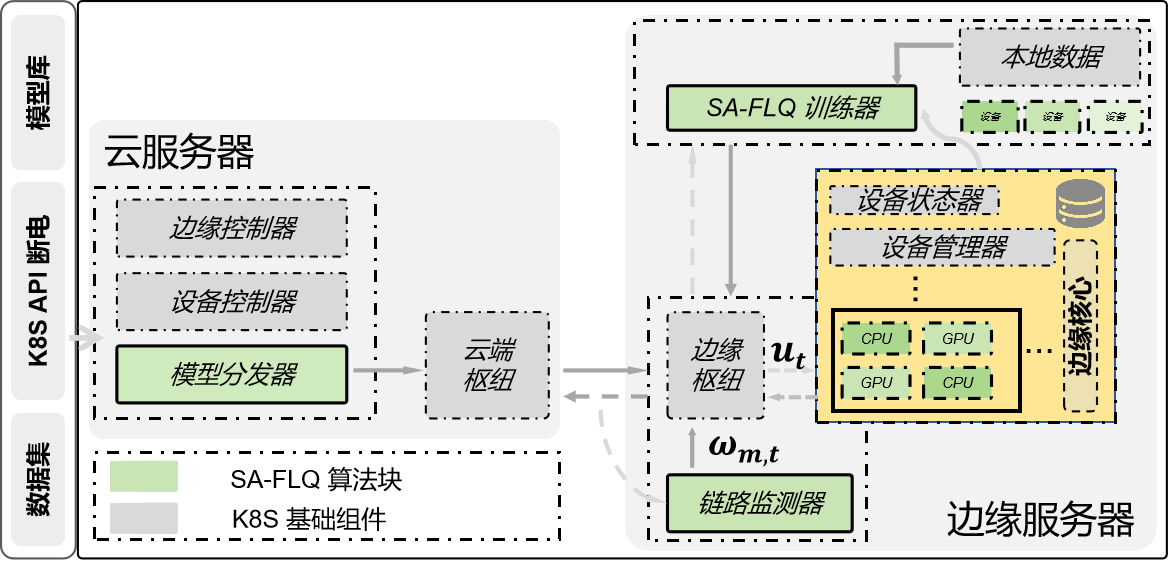
\includegraphics[width=0.95\textwidth]{system_architecture.png}
\caption{System-level deployment architecture of SA-FLQ on a K8s and KubeEdge based edge cluster. Green boxes indicate SA-FLQ enhancement modules developed for maritime DIL environments, while gray boxes represent KubeEdge base components. The server runs CloudCore with model distributor and quantizer modules. Edge nodes run EdgeCore with link monitoring, device twin synchronization, and SA-FLQ trainer containers. The full system maintains a sense-decide-execute-writeback closed loop.}
\label{fig:system_architecture}
\end{figure*}

\subsubsection{Detection Results}
Fig.~\ref{fig:oil_detection} presents sample detection results. The model correctly identifies oil-covered areas with tight bounding boxes.

\begin{figure}[!t]
\centering
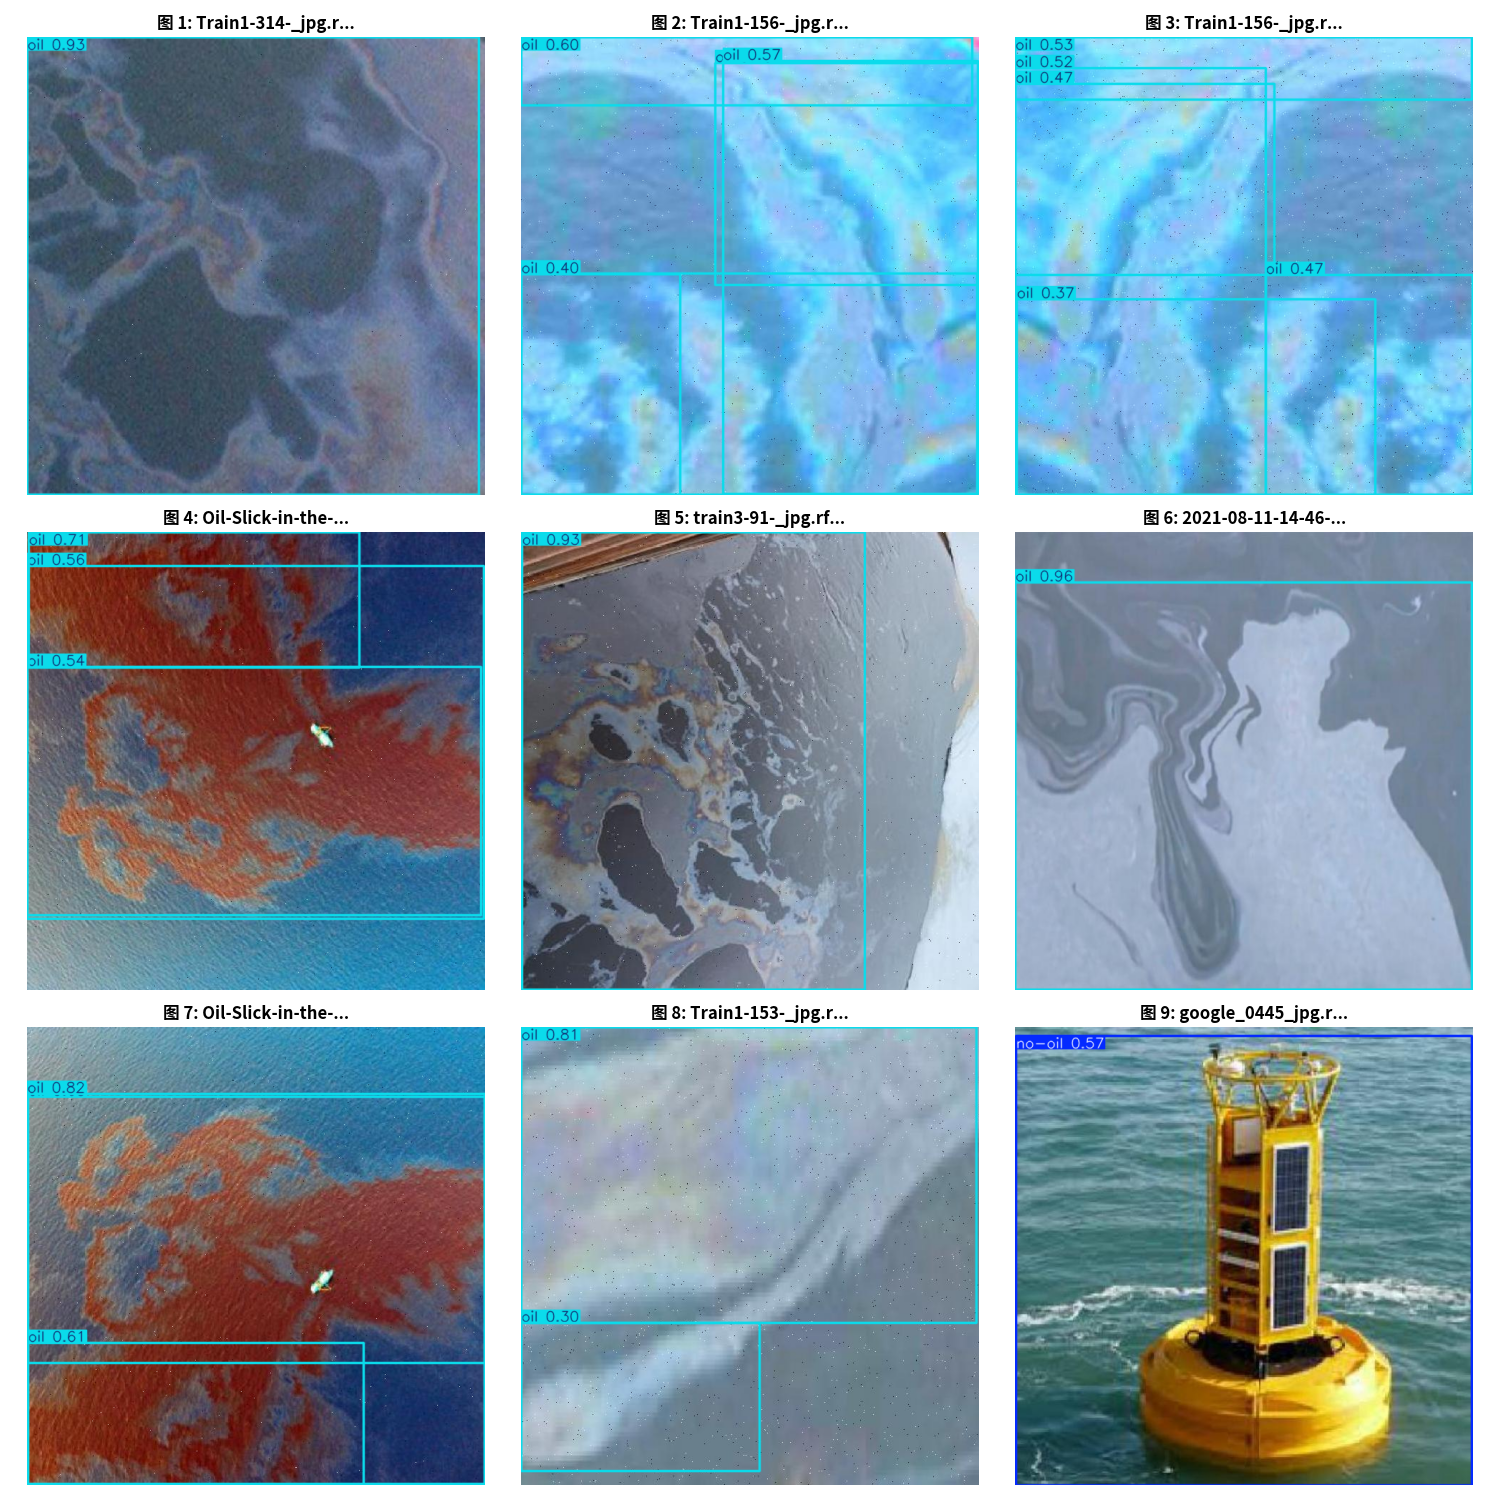
\includegraphics[width=\columnwidth]{oil_detection_vis.png}
\caption{Representative qualitative results of the federated oil spill detection task. The figure displays detection performance under various sea conditions including wave disturbance, low light, and strong reflection. Blue boxes indicate detected oil spill areas with confidence scores. Results demonstrate the good generalization and robustness of the SA-FLQ trained model across diverse maritime scenarios.}
\label{fig:oil_detection}
\end{figure}

\subsubsection{Quantitative Performance}
Table~\ref{tab:communication} provides a comprehensive comparison of communication efficiency and detection performance.

\begin{table}[!t]
\caption{Communication Efficiency and Detection Performance on Oil Spill Dataset}
\label{tab:communication}
\centering
\begin{tabular}{lcccc}
\toprule
\textbf{Method} & \textbf{Upload/Round} & \textbf{Compression} & \textbf{mAP50} & \textbf{mAP50-95} \\
\midrule
FedAvg (FP32) & 0.29 Gbit & $1.0\times$ & 0.830 & 0.512 \\
QSGD (8-bit) & 0.07 Gbit & $4.0\times$ & 0.798 & 0.484 \\
LAQ (4-bit) & 0.04 Gbit & $7.3\times$ & 0.785 & 0.471 \\
\midrule
SA-FLQ (8-bit) & 0.07 Gbit & $4.0\times$ & 0.822 & 0.503 \\
SA-FLQ (4-bit) & 0.04 Gbit & $7.3\times$ & 0.815 & 0.495 \\
SA-FLQ (2-bit) & 0.02 Gbit & $14.5\times$ & 0.793 & 0.478 \\
SA-FLQ (1-bit) & 0.01 Gbit & $29.0\times$ & 0.780 & 0.461 \\
\bottomrule
\end{tabular}
\end{table}

SA-FLQ with 8-bit quantization achieves mAP50 of 0.822, only $0.8\%$ below the full-precision baseline. With 4-bit quantization, mAP50 remains at 0.815, which is acceptable for most practical applications while achieving $7.3\times$ compression.

\begin{figure}[!t]
\centering
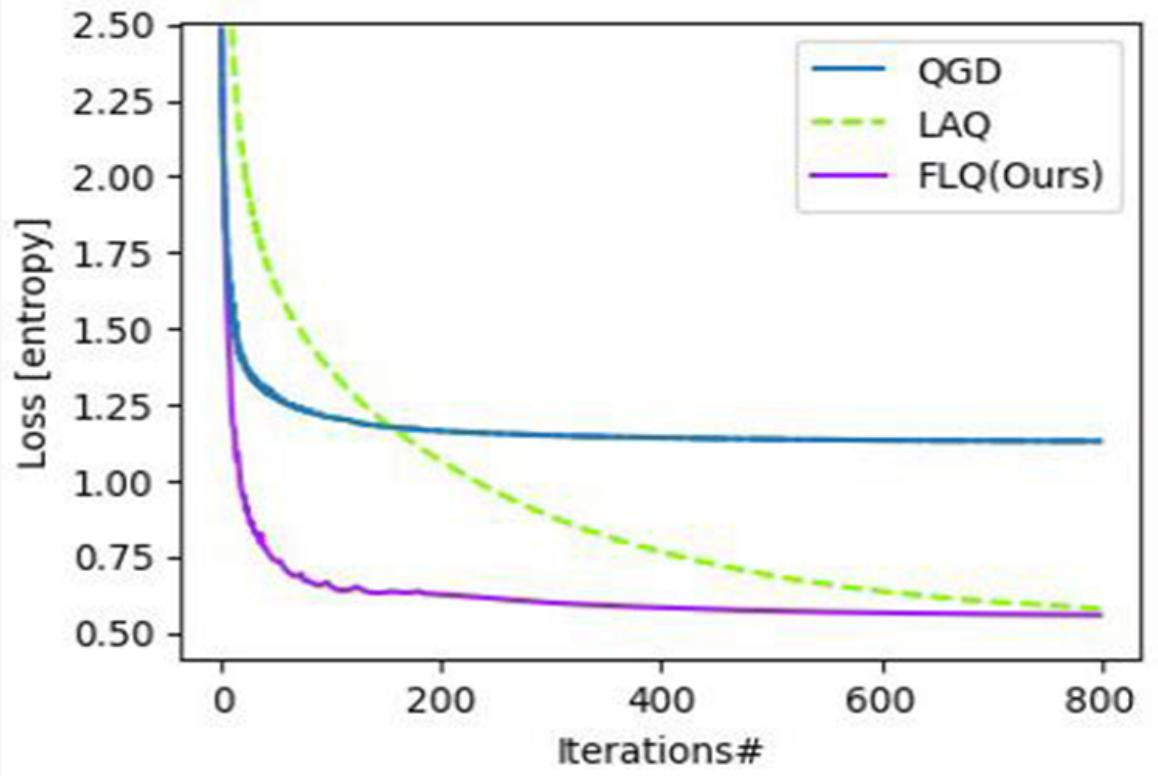
\includegraphics[width=0.9\columnwidth]{average_result.jpg}
\caption{Communication efficiency vs detection accuracy comparison. SA-FLQ dominates the Pareto frontier, achieving superior accuracy at all compression levels.}
\label{fig:avg_result}
\end{figure}

% ============================================================
%                    VI. CONCLUSION
% ============================================================
\section{Conclusion}
\label{sec:conclusion}

In this paper, we proposed SA-FLQ (System-Aware Federated Low-bitwidth Quantization), a communication-efficient federated learning framework designed for maritime edge computing under DIL (Disconnected, Intermittent, Low-bandwidth) conditions. We introduced the KEW (KubeEdge Wireless) platform architecture, a three-layer edge system that establishes standardized observable variables (bandwidth, latency, energy) and controllable variables (client selection, local epochs, quantization bitwidth) as a unified system interface. Based on this architecture, SA-FLQ dynamically adjusts quantization strategies through a sense-decide-execute-writeback closed-loop mechanism, achieving joint optimization of communication overhead, computation latency, and model accuracy.

Theoretical analysis established convergence guarantees for SA-FLQ under quantization noise. Extensive experiments on simulation benchmarks and a real-world oil spill detection task deployed on a Kubernetes-based Jetson edge cluster demonstrated that SA-FLQ achieves up to $7.3\times$ communication compression with less than $1\%$ accuracy degradation and $86\%$ per-round latency reduction compared to full-precision federated averaging.

Future work will explore reinforcement learning-based adaptive bit selection and integration with heterogeneous maritime networks including satellite-UAV-terrestrial links.

% ============================================================
%                    ACKNOWLEDGMENT
% ============================================================
\section*{Acknowledgment}
This work was supported in part by the National Natural Science Foundation of China.

% ============================================================
%                    REFERENCES
% ============================================================
\bibliographystyle{IEEEtran}
\bibliography{Marine_Edge}

\end{document}
